\PassOptionsToPackage{unicode=true}{hyperref} % options for packages loaded elsewhere
\PassOptionsToPackage{hyphens}{url}
%
\documentclass[]{article}
\usepackage{lmodern}
\usepackage{amssymb,amsmath}
\usepackage{ifxetex,ifluatex}
\usepackage{fixltx2e} % provides \textsubscript
\ifnum 0\ifxetex 1\fi\ifluatex 1\fi=0 % if pdftex
  \usepackage[T1]{fontenc}
  \usepackage[utf8]{inputenc}
  \usepackage{textcomp} % provides euro and other symbols
\else % if luatex or xelatex
  \usepackage{unicode-math}
  \defaultfontfeatures{Ligatures=TeX,Scale=MatchLowercase}
\fi
% use upquote if available, for straight quotes in verbatim environments
\IfFileExists{upquote.sty}{\usepackage{upquote}}{}
% use microtype if available
\IfFileExists{microtype.sty}{%
\usepackage[]{microtype}
\UseMicrotypeSet[protrusion]{basicmath} % disable protrusion for tt fonts
}{}
\IfFileExists{parskip.sty}{%
\usepackage{parskip}
}{% else
\setlength{\parindent}{0pt}
\setlength{\parskip}{6pt plus 2pt minus 1pt}
}
\usepackage{hyperref}
\hypersetup{
            pdfauthor={Joaquín Moreno1,3; Sergio Asensio3; Miguel Berdugo3,4; Beatriz Gozalo3; Victoria Ochoa3; Blas M. Benito3,2; Fernando T. Maestre3,5},
            pdfborder={0 0 0},
            breaklinks=true}
\urlstyle{same}  % don't use monospace font for urls
\usepackage[margin=1in]{geometry}
\usepackage{color}
\usepackage{fancyvrb}
\newcommand{\VerbBar}{|}
\newcommand{\VERB}{\Verb[commandchars=\\\{\}]}
\DefineVerbatimEnvironment{Highlighting}{Verbatim}{commandchars=\\\{\}}
% Add ',fontsize=\small' for more characters per line
\usepackage{framed}
\definecolor{shadecolor}{RGB}{248,248,248}
\newenvironment{Shaded}{\begin{snugshade}}{\end{snugshade}}
\newcommand{\AlertTok}[1]{\textcolor[rgb]{0.94,0.16,0.16}{#1}}
\newcommand{\AnnotationTok}[1]{\textcolor[rgb]{0.56,0.35,0.01}{\textbf{\textit{#1}}}}
\newcommand{\AttributeTok}[1]{\textcolor[rgb]{0.77,0.63,0.00}{#1}}
\newcommand{\BaseNTok}[1]{\textcolor[rgb]{0.00,0.00,0.81}{#1}}
\newcommand{\BuiltInTok}[1]{#1}
\newcommand{\CharTok}[1]{\textcolor[rgb]{0.31,0.60,0.02}{#1}}
\newcommand{\CommentTok}[1]{\textcolor[rgb]{0.56,0.35,0.01}{\textit{#1}}}
\newcommand{\CommentVarTok}[1]{\textcolor[rgb]{0.56,0.35,0.01}{\textbf{\textit{#1}}}}
\newcommand{\ConstantTok}[1]{\textcolor[rgb]{0.00,0.00,0.00}{#1}}
\newcommand{\ControlFlowTok}[1]{\textcolor[rgb]{0.13,0.29,0.53}{\textbf{#1}}}
\newcommand{\DataTypeTok}[1]{\textcolor[rgb]{0.13,0.29,0.53}{#1}}
\newcommand{\DecValTok}[1]{\textcolor[rgb]{0.00,0.00,0.81}{#1}}
\newcommand{\DocumentationTok}[1]{\textcolor[rgb]{0.56,0.35,0.01}{\textbf{\textit{#1}}}}
\newcommand{\ErrorTok}[1]{\textcolor[rgb]{0.64,0.00,0.00}{\textbf{#1}}}
\newcommand{\ExtensionTok}[1]{#1}
\newcommand{\FloatTok}[1]{\textcolor[rgb]{0.00,0.00,0.81}{#1}}
\newcommand{\FunctionTok}[1]{\textcolor[rgb]{0.00,0.00,0.00}{#1}}
\newcommand{\ImportTok}[1]{#1}
\newcommand{\InformationTok}[1]{\textcolor[rgb]{0.56,0.35,0.01}{\textbf{\textit{#1}}}}
\newcommand{\KeywordTok}[1]{\textcolor[rgb]{0.13,0.29,0.53}{\textbf{#1}}}
\newcommand{\NormalTok}[1]{#1}
\newcommand{\OperatorTok}[1]{\textcolor[rgb]{0.81,0.36,0.00}{\textbf{#1}}}
\newcommand{\OtherTok}[1]{\textcolor[rgb]{0.56,0.35,0.01}{#1}}
\newcommand{\PreprocessorTok}[1]{\textcolor[rgb]{0.56,0.35,0.01}{\textit{#1}}}
\newcommand{\RegionMarkerTok}[1]{#1}
\newcommand{\SpecialCharTok}[1]{\textcolor[rgb]{0.00,0.00,0.00}{#1}}
\newcommand{\SpecialStringTok}[1]{\textcolor[rgb]{0.31,0.60,0.02}{#1}}
\newcommand{\StringTok}[1]{\textcolor[rgb]{0.31,0.60,0.02}{#1}}
\newcommand{\VariableTok}[1]{\textcolor[rgb]{0.00,0.00,0.00}{#1}}
\newcommand{\VerbatimStringTok}[1]{\textcolor[rgb]{0.31,0.60,0.02}{#1}}
\newcommand{\WarningTok}[1]{\textcolor[rgb]{0.56,0.35,0.01}{\textbf{\textit{#1}}}}
\usepackage{graphicx,grffile}
\makeatletter
\def\maxwidth{\ifdim\Gin@nat@width>\linewidth\linewidth\else\Gin@nat@width\fi}
\def\maxheight{\ifdim\Gin@nat@height>\textheight\textheight\else\Gin@nat@height\fi}
\makeatother
% Scale images if necessary, so that they will not overflow the page
% margins by default, and it is still possible to overwrite the defaults
% using explicit options in \includegraphics[width, height, ...]{}
\setkeys{Gin}{width=\maxwidth,height=\maxheight,keepaspectratio}
\setlength{\emergencystretch}{3em}  % prevent overfull lines
\providecommand{\tightlist}{%
  \setlength{\itemsep}{0pt}\setlength{\parskip}{0pt}}
\setcounter{secnumdepth}{5}
% Redefines (sub)paragraphs to behave more like sections
\ifx\paragraph\undefined\else
\let\oldparagraph\paragraph
\renewcommand{\paragraph}[1]{\oldparagraph{#1}\mbox{}}
\fi
\ifx\subparagraph\undefined\else
\let\oldsubparagraph\subparagraph
\renewcommand{\subparagraph}[1]{\oldsubparagraph{#1}\mbox{}}
\fi

% set default figure placement to htbp
\makeatletter
\def\fps@figure{htbp}
\makeatother

\usepackage{booktabs}
\usepackage[table]{xcolor}
\usepackage{color}
\usepackage{fontspec}
\setmainfont[Scale=1.1]{Open Sans}
\setmonofont[Scale=0.9]{Open Sans}
\linespread{1.3}
\usepackage{listings}
\lstset{breaklines=true}

\usepackage{float}
\let\origfigure\figure
\let\endorigfigure\endfigure
\renewenvironment{figure}[1][2] {
    \expandafter\origfigure\expandafter[H]
} {
    \endorigfigure
}

\floatplacement{figure}{H}

\usepackage{pdflscape}
\newcommand{\blandscape}{\begin{landscape}}
\newcommand{\elandscape}{\end{landscape}}

\usepackage{caption} 
\captionsetup[table]{skip=10pt}
\usepackage[tableposition=above]{caption}

\title{The MOISCRUST dataset:\\
a spatio-temporal continuous soil moisture dataset\\
from a Mediterranean semiarid dryland\\
from 2006 to 2020\\
SUPPLEMENTARY MATERIAL}
\author{Joaquín Moreno\textsuperscript{1,3} \and Sergio Asensio\textsuperscript{3} \and Miguel Berdugo\textsuperscript{3,4} \and Beatriz Gozalo\textsuperscript{3} \and Victoria Ochoa\textsuperscript{3} \and Blas M. Benito\textsuperscript{3,2} \and Fernando T. Maestre\textsuperscript{3,5}}
\date{}

\begin{document}
\maketitle

{
\setcounter{tocdepth}{1}
\tableofcontents
}
\textsuperscript{1} Corresponding author, e-mail:
\href{mailto:joaquin.moreno@ua.es}{\nolinkurl{joaquin.moreno@ua.es}}\\
\textsuperscript{2} Code and workflow design.\\
\textsuperscript{3} Instituto Multidisciplinar para el Estudio del Medio
``Ramon Margalef'', Universidad de Alicante, Edificio Nuevos Institutos,
Carretera de San Vicente del Raspeig s/n, 03690 San Vicente del Raspeig,
Spain.\\
\textsuperscript{4} Institut Department of Environmental Systems
Science, ETH Zürich. Universitätstrasse 16, 8092 Zurich, Switzerland.\\
\textsuperscript{5} Departamento de Ecología, Universidad de Alicante,
Carretera de San Vicente del Raspeig s/n, 03690 San Vicente del Raspeig,
Alicante, Spain.

\newpage

\hypertarget{summary}{%
\section{Summary}\label{summary}}

The \textbf{MOISCRUST} database contains volumetric water content (VWC,
m³/m³) measures taken by soil moisture sensors EC-5, Decagon Devices
Inc., Pullman, USA) every 120 minutes (17th November 2006 to 31th
January 2017) and 150 minutes (1st February 2017 to 16th December 2020)
from three replicates in five different microsites (\emph{Stipa}
tussocks, \emph{Retama} shrubs, and areas with low, medium and high
cover of biocrust-forming lichens) located in The Aranjuez Experimental
Station (central Iberian Peninsula, 40⁰02' N, 3⁰32'W; 590 m.a.s.l).
During the long time-span these sensors have been working, there have
been periods when data capture has not possible due to technical issues,
and as consequence, 34.63\% of the database records are missing entries.
This reproducible workflow describes in detail the method used to impute
missing data in the \textbf{MOISCRUST} database.

The \textbf{MOISCRUST} database and this reproducible document are
distributed under the license
\href{https://creativecommons.org/licenses/by/4.0/legalcode}{\texttt{Creative\ Commons\ Attribution-NonCommercial-ShareAlike\ 4.0\ International}}.

\hypertarget{reproducing-this-workflow}{%
\section{Reproducing this workflow}\label{reproducing-this-workflow}}

This reproducible workflow is available as an interactive Rstudio
notebook in the file \textbf{moiscrust.Rmd} stored in this repository.
It is packaged with \href{https://cran.r-project.org/package=renv}{renv}
to facilitate reproducibility. To run it in your computer, execute the
code chunk below to prepare the session. You will need to replace
\texttt{r}eval = TRUE\texttt{with}r \texttt{eval\ =\ TRUE} in the header
of the code chunk.

\begin{Shaded}
\begin{Highlighting}[]
\KeywordTok{install.packages}\NormalTok{(}\StringTok{"renv"}\NormalTok{)}
\KeywordTok{library}\NormalTok{(renv)}
\NormalTok{renv}\OperatorTok{::}\KeywordTok{restore}\NormalTok{()}
\end{Highlighting}
\end{Shaded}

\hypertarget{data-loading-and-preparation}{%
\section{Data loading and
preparation}\label{data-loading-and-preparation}}

\hypertarget{installing-and-loading-the-required-libraries}{%
\subsection{Installing and loading the required
libraries}\label{installing-and-loading-the-required-libraries}}

The following libraries are required to run this workflow. These are
already installed in the local \textbf{renv} folder, so there is no need
to install them if they are not available in your computer.

\begin{Shaded}
\begin{Highlighting}[]
\CommentTok{#automatic install of packages if they are not readily available}
\NormalTok{required_packages <-}\StringTok{ }\KeywordTok{c}\NormalTok{(}
  \StringTok{"data.table"}\NormalTok{,}
  \StringTok{"tidyverse"}\NormalTok{,}
  \StringTok{"kableExtra"}\NormalTok{,}
  \StringTok{"foreach"}\NormalTok{,}
  \StringTok{"doParallel"}\NormalTok{,}
  \StringTok{"readr"}\NormalTok{,}
  \StringTok{"writexl"}\NormalTok{,}
  \StringTok{"RSQLite"}\NormalTok{,}
  \StringTok{"zip"}\NormalTok{,}
  \StringTok{"knitr"}\NormalTok{,}
  \StringTok{"DBI"}
\NormalTok{)}

\CommentTok{#loading packages}
\KeywordTok{invisible}\NormalTok{(}
  \KeywordTok{lapply}\NormalTok{(}
\NormalTok{    required_packages, }
\NormalTok{    library, }
    \DataTypeTok{character.only =} \OtherTok{TRUE}
\NormalTok{    )}
\NormalTok{  )}

\CommentTok{#knitr options}
\NormalTok{knitr}\OperatorTok{::}\NormalTok{opts_chunk}\OperatorTok{$}\KeywordTok{set}\NormalTok{(}\DataTypeTok{echo =} \OtherTok{TRUE}\NormalTok{, }\DataTypeTok{warning =} \OtherTok{FALSE}\NormalTok{, }\DataTypeTok{message =} \OtherTok{FALSE}\NormalTok{)}
\NormalTok{knitr}\OperatorTok{::}\NormalTok{knit_hooks}\OperatorTok{$}\KeywordTok{set}\NormalTok{(}\DataTypeTok{document =} \ControlFlowTok{function}\NormalTok{(x) \{}\KeywordTok{sub}\NormalTok{(}\StringTok{'}\CharTok{\textbackslash{}\textbackslash{}}\StringTok{usepackage\{xcolor\}'}\NormalTok{, }\StringTok{'}\CharTok{\textbackslash{}\textbackslash{}}\StringTok{usepackage\{xcolor\}'}\NormalTok{, x, }\DataTypeTok{fixed =} \OtherTok{TRUE}\NormalTok{)\})}

\CommentTok{#removing objects}
\KeywordTok{rm}\NormalTok{(required_packages)}
\end{Highlighting}
\end{Shaded}

\hypertarget{loading-and-preparing-the-raw-data}{%
\subsection{Loading and preparing the raw
data}\label{loading-and-preparing-the-raw-data}}

The raw data, stored in the file \emph{moiscrust\_raw.csv} was compiled
by the members of \href{https://maestrelab.com/en/}{Maestre Lab} from
the data provided by the soil moisture sensors.

\begin{Shaded}
\begin{Highlighting}[]
\CommentTok{#load, clean names, and rename time columns}
\NormalTok{moiscrust <-}\StringTok{ }\NormalTok{data.table}\OperatorTok{::}\KeywordTok{fread}\NormalTok{(}\DataTypeTok{file =} \StringTok{"moiscrust_raw.csv"}\NormalTok{) }\OperatorTok\StringTok{ }
\StringTok{  }\KeywordTok{as.data.frame}\NormalTok{()}
\end{Highlighting}
\end{Shaded}

\begin{table}[H]
\centering
\resizebox{\linewidth}{!}{
\begin{tabular}[t]{l|l|r|r|r|r|r|r|r|r|r|r|r|r|r|r|r}
\hline
date & time & retama\_1 & retama\_2 & retama\_3 & stipa\_1 & stipa\_2 & stipa\_3 & bare\_soil\_1 & bare\_soil\_2 & bare\_soil\_3 & biocrust\_medium\_1 & biocrust\_medium\_2 & biocrust\_medium\_3 & biocrust\_high\_1 & biocrust\_high\_2 & biocrust\_high\_3\\
\hline
\cellcolor{gray!6}{17/11/2006} & \cellcolor{gray!6}{18:00:00} & \cellcolor{gray!6}{0.197} & \cellcolor{gray!6}{NA} & \cellcolor{gray!6}{NA} & \cellcolor{gray!6}{0.132} & \cellcolor{gray!6}{NA} & \cellcolor{gray!6}{NA} & \cellcolor{gray!6}{0.232} & \cellcolor{gray!6}{NA} & \cellcolor{gray!6}{NA} & \cellcolor{gray!6}{0.205} & \cellcolor{gray!6}{NA} & \cellcolor{gray!6}{NA} & \cellcolor{gray!6}{0.121} & \cellcolor{gray!6}{NA} & \cellcolor{gray!6}{NA}\\
\hline
17/11/2006 & 20:00:00 & 0.195 & NA & NA & 0.131 & NA & NA & 0.233 & NA & NA & 0.203 & NA & NA & 0.117 & NA & NA\\
\hline
\cellcolor{gray!6}{17/11/2006} & \cellcolor{gray!6}{22:00:00} & \cellcolor{gray!6}{0.194} & \cellcolor{gray!6}{NA} & \cellcolor{gray!6}{NA} & \cellcolor{gray!6}{0.131} & \cellcolor{gray!6}{NA} & \cellcolor{gray!6}{NA} & \cellcolor{gray!6}{0.234} & \cellcolor{gray!6}{NA} & \cellcolor{gray!6}{NA} & \cellcolor{gray!6}{0.203} & \cellcolor{gray!6}{NA} & \cellcolor{gray!6}{NA} & \cellcolor{gray!6}{0.117} & \cellcolor{gray!6}{NA} & \cellcolor{gray!6}{NA}\\
\hline
18/11/2006 & 0:00:00 & 0.194 & NA & NA & 0.131 & NA & NA & 0.234 & NA & NA & 0.203 & NA & NA & 0.116 & NA & NA\\
\hline
\cellcolor{gray!6}{18/11/2006} & \cellcolor{gray!6}{2:00:00} & \cellcolor{gray!6}{0.194} & \cellcolor{gray!6}{NA} & \cellcolor{gray!6}{NA} & \cellcolor{gray!6}{0.130} & \cellcolor{gray!6}{NA} & \cellcolor{gray!6}{NA} & \cellcolor{gray!6}{0.234} & \cellcolor{gray!6}{NA} & \cellcolor{gray!6}{NA} & \cellcolor{gray!6}{0.203} & \cellcolor{gray!6}{NA} & \cellcolor{gray!6}{NA} & \cellcolor{gray!6}{0.116} & \cellcolor{gray!6}{NA} & \cellcolor{gray!6}{NA}\\
\hline
18/11/2006 & 4:00:00 & 0.194 & NA & NA & 0.130 & NA & NA & 0.234 & NA & NA & 0.202 & NA & NA & 0.116 & NA & NA\\
\hline
\cellcolor{gray!6}{18/11/2006} & \cellcolor{gray!6}{6:00:00} & \cellcolor{gray!6}{0.194} & \cellcolor{gray!6}{NA} & \cellcolor{gray!6}{NA} & \cellcolor{gray!6}{0.130} & \cellcolor{gray!6}{NA} & \cellcolor{gray!6}{NA} & \cellcolor{gray!6}{0.234} & \cellcolor{gray!6}{NA} & \cellcolor{gray!6}{NA} & \cellcolor{gray!6}{0.202} & \cellcolor{gray!6}{NA} & \cellcolor{gray!6}{NA} & \cellcolor{gray!6}{0.115} & \cellcolor{gray!6}{NA} & \cellcolor{gray!6}{NA}\\
\hline
18/11/2006 & 8:00:00 & 0.194 & NA & NA & 0.130 & NA & NA & 0.234 & NA & NA & 0.202 & NA & NA & 0.115 & NA & NA\\
\hline
\cellcolor{gray!6}{18/11/2006} & \cellcolor{gray!6}{10:00:00} & \cellcolor{gray!6}{0.194} & \cellcolor{gray!6}{NA} & \cellcolor{gray!6}{NA} & \cellcolor{gray!6}{0.130} & \cellcolor{gray!6}{NA} & \cellcolor{gray!6}{NA} & \cellcolor{gray!6}{0.234} & \cellcolor{gray!6}{NA} & \cellcolor{gray!6}{NA} & \cellcolor{gray!6}{0.202} & \cellcolor{gray!6}{NA} & \cellcolor{gray!6}{NA} & \cellcolor{gray!6}{0.115} & \cellcolor{gray!6}{NA} & \cellcolor{gray!6}{NA}\\
\hline
18/11/2006 & 12:00:00 & 0.194 & NA & NA & 0.130 & NA & NA & 0.234 & NA & NA & 0.202 & NA & NA & 0.116 & NA & NA\\
\hline
\cellcolor{gray!6}{18/11/2006} & \cellcolor{gray!6}{14:00:00} & \cellcolor{gray!6}{0.195} & \cellcolor{gray!6}{NA} & \cellcolor{gray!6}{NA} & \cellcolor{gray!6}{0.131} & \cellcolor{gray!6}{NA} & \cellcolor{gray!6}{NA} & \cellcolor{gray!6}{0.234} & \cellcolor{gray!6}{NA} & \cellcolor{gray!6}{NA} & \cellcolor{gray!6}{0.202} & \cellcolor{gray!6}{NA} & \cellcolor{gray!6}{NA} & \cellcolor{gray!6}{0.116} & \cellcolor{gray!6}{NA} & \cellcolor{gray!6}{NA}\\
\hline
18/11/2006 & 16:00:00 & 0.195 & NA & NA & 0.131 & NA & NA & 0.233 & NA & NA & 0.201 & NA & NA & 0.115 & NA & NA\\
\hline
\cellcolor{gray!6}{18/11/2006} & \cellcolor{gray!6}{18:00:00} & \cellcolor{gray!6}{0.194} & \cellcolor{gray!6}{NA} & \cellcolor{gray!6}{NA} & \cellcolor{gray!6}{0.130} & \cellcolor{gray!6}{NA} & \cellcolor{gray!6}{NA} & \cellcolor{gray!6}{0.233} & \cellcolor{gray!6}{NA} & \cellcolor{gray!6}{NA} & \cellcolor{gray!6}{0.200} & \cellcolor{gray!6}{NA} & \cellcolor{gray!6}{NA} & \cellcolor{gray!6}{0.114} & \cellcolor{gray!6}{NA} & \cellcolor{gray!6}{NA}\\
\hline
18/11/2006 & 20:00:00 & 0.193 & NA & NA & 0.129 & NA & NA & 0.233 & NA & NA & 0.199 & NA & NA & 0.112 & NA & NA\\
\hline
\cellcolor{gray!6}{18/11/2006} & \cellcolor{gray!6}{22:00:00} & \cellcolor{gray!6}{0.192} & \cellcolor{gray!6}{NA} & \cellcolor{gray!6}{NA} & \cellcolor{gray!6}{0.129} & \cellcolor{gray!6}{NA} & \cellcolor{gray!6}{NA} & \cellcolor{gray!6}{0.234} & \cellcolor{gray!6}{NA} & \cellcolor{gray!6}{NA} & \cellcolor{gray!6}{0.199} & \cellcolor{gray!6}{NA} & \cellcolor{gray!6}{NA} & \cellcolor{gray!6}{0.111} & \cellcolor{gray!6}{NA} & \cellcolor{gray!6}{NA}\\
\hline
19/11/2006 & 0:00:00 & 0.192 & NA & NA & 0.128 & NA & NA & 0.234 & NA & NA & 0.199 & NA & NA & 0.111 & NA & NA\\
\hline
\cellcolor{gray!6}{19/11/2006} & \cellcolor{gray!6}{2:00:00} & \cellcolor{gray!6}{0.191} & \cellcolor{gray!6}{NA} & \cellcolor{gray!6}{NA} & \cellcolor{gray!6}{0.128} & \cellcolor{gray!6}{NA} & \cellcolor{gray!6}{NA} & \cellcolor{gray!6}{0.234} & \cellcolor{gray!6}{NA} & \cellcolor{gray!6}{NA} & \cellcolor{gray!6}{0.198} & \cellcolor{gray!6}{NA} & \cellcolor{gray!6}{NA} & \cellcolor{gray!6}{0.110} & \cellcolor{gray!6}{NA} & \cellcolor{gray!6}{NA}\\
\hline
19/11/2006 & 4:00:00 & 0.190 & NA & NA & 0.127 & NA & NA & 0.234 & NA & NA & 0.198 & NA & NA & 0.109 & NA & NA\\
\hline
\cellcolor{gray!6}{19/11/2006} & \cellcolor{gray!6}{6:00:00} & \cellcolor{gray!6}{0.189} & \cellcolor{gray!6}{NA} & \cellcolor{gray!6}{NA} & \cellcolor{gray!6}{0.127} & \cellcolor{gray!6}{NA} & \cellcolor{gray!6}{NA} & \cellcolor{gray!6}{0.234} & \cellcolor{gray!6}{NA} & \cellcolor{gray!6}{NA} & \cellcolor{gray!6}{0.198} & \cellcolor{gray!6}{NA} & \cellcolor{gray!6}{NA} & \cellcolor{gray!6}{0.109} & \cellcolor{gray!6}{NA} & \cellcolor{gray!6}{NA}\\
\hline
19/11/2006 & 8:00:00 & 0.188 & NA & NA & 0.127 & NA & NA & 0.234 & NA & NA & 0.198 & NA & NA & 0.109 & NA & NA\\
\hline
\end{tabular}}
\end{table}

\hypertarget{formatting-dates-and-times}{%
\subsection{Formatting dates and
times}\label{formatting-dates-and-times}}

The raw data contains two fields representing time, namely \emph{date}
(year, month, and day), and \emph{time} (hour, minute, and seconds).
Below we format these fields according to the POSIX standard, and add
new fields adding criteria to subset the data by time:

\begin{itemize}
\tightlist
\item
  \emph{date\_time}: Date and time in POSIX format.
\item
  \emph{date\_time\_id}: Unique identificator for each
  \emph{date\_time}.
\item
  \emph{year}: Year number.
\item
  \emph{year\_day}: Day of the year.
\item
  \emph{month}: Month number.
\item
  \emph{month\_day}: Day of the month.
\item
  \emph{week}: Week of the year.
\item
  \emph{week\_day}: Day of the week.
\end{itemize}

\begin{Shaded}
\begin{Highlighting}[]
\CommentTok{#date to Year-month-day}
\NormalTok{moiscrust}\OperatorTok{$}\NormalTok{date <-}\StringTok{ }\KeywordTok{format}\NormalTok{(}
  \KeywordTok{as.POSIXct}\NormalTok{(}
    \KeywordTok{strptime}\NormalTok{(}
\NormalTok{      moiscrust}\OperatorTok{$}\NormalTok{date,}
      \StringTok{"%d/%m/%Y"}\NormalTok{,}
      \DataTypeTok{tz =} \StringTok{""}
\NormalTok{      )}
\NormalTok{    ),}
  \DataTypeTok{format =} \StringTok{"%Y-%m-%d"}
\NormalTok{  )}

\CommentTok{#time to Hour-Minute}
\NormalTok{moiscrust}\OperatorTok{$}\NormalTok{time <-}\StringTok{ }\KeywordTok{format}\NormalTok{(}
  \KeywordTok{as.POSIXct}\NormalTok{(}
    \KeywordTok{strptime}\NormalTok{(}
\NormalTok{      moiscrust}\OperatorTok{$}\NormalTok{time,}
      \StringTok{"%H:%M:%S"}\NormalTok{,}
      \DataTypeTok{tz =} \StringTok{""}
\NormalTok{      )}
\NormalTok{    ),}
  \DataTypeTok{format =} \StringTok{"%H:%M"}
\NormalTok{  )}

\CommentTok{#joining date and time}
\NormalTok{moiscrust}\OperatorTok{$}\NormalTok{date_time <-}\StringTok{ }\KeywordTok{as.POSIXct}\NormalTok{(}
  \KeywordTok{paste}\NormalTok{(}
\NormalTok{    moiscrust}\OperatorTok{$}\NormalTok{date, }
\NormalTok{    moiscrust}\OperatorTok{$}\NormalTok{time}
\NormalTok{    ), }
  \DataTypeTok{format=}\StringTok{"%Y-%m-%d %H:%M"}
\NormalTok{  )}

\CommentTok{#unique id for each observation}
\NormalTok{moiscrust}\OperatorTok{$}\NormalTok{date_time_id <-}\StringTok{ }\DecValTok{1}\OperatorTok{:}\KeywordTok{nrow}\NormalTok{(moiscrust)}

\CommentTok{#creating year, month, and day related columns}
\NormalTok{moiscrust}\OperatorTok{$}\NormalTok{year <-}\StringTok{ }\NormalTok{lubridate}\OperatorTok{::}\KeywordTok{year}\NormalTok{(moiscrust}\OperatorTok{$}\NormalTok{date)}
\NormalTok{moiscrust}\OperatorTok{$}\NormalTok{year_day <-}\StringTok{ }\NormalTok{lubridate}\OperatorTok{::}\KeywordTok{yday}\NormalTok{(moiscrust}\OperatorTok{$}\NormalTok{date)}
\NormalTok{moiscrust}\OperatorTok{$}\NormalTok{month <-}\StringTok{ }\NormalTok{lubridate}\OperatorTok{::}\KeywordTok{month}\NormalTok{(moiscrust}\OperatorTok{$}\NormalTok{date)}
\NormalTok{moiscrust}\OperatorTok{$}\NormalTok{month_day <-}\StringTok{ }\NormalTok{lubridate}\OperatorTok{::}\KeywordTok{mday}\NormalTok{(moiscrust}\OperatorTok{$}\NormalTok{date)}
\NormalTok{moiscrust}\OperatorTok{$}\NormalTok{week <-}\StringTok{ }\NormalTok{lubridate}\OperatorTok{::}\KeywordTok{week}\NormalTok{(moiscrust}\OperatorTok{$}\NormalTok{date)}
\NormalTok{moiscrust}\OperatorTok{$}\NormalTok{week_day <-}\StringTok{ }\NormalTok{lubridate}\OperatorTok{::}\KeywordTok{wday}\NormalTok{(moiscrust}\OperatorTok{$}\NormalTok{date)}
\end{Highlighting}
\end{Shaded}

\hypertarget{reordering-time-and-data-columns-and-arranging-the-data-into-long-format}{%
\subsection{Reordering time and data columns and arranging the data into
long
format}\label{reordering-time-and-data-columns-and-arranging-the-data-into-long-format}}

At this point, the \emph{MOISCRUST} data has 15 columns representing
soils moisture measures (microsites per three replicates per microsite),
and 10 columns representing \emph{time}. The data is also structured in
what is known as a
\href{https://sejdemyr.github.io/r-tutorials/basics/wide-and-long/}{``wide
format''}. Below we reorder these columns to facilitate arranging the
data into a ``long format''.

\begin{Shaded}
\begin{Highlighting}[]
\CommentTok{#names of the sensors}
\NormalTok{sensors <-}\StringTok{ }\KeywordTok{c}\NormalTok{(}
  \StringTok{"retama_1"}\NormalTok{,}
  \StringTok{"retama_2"}\NormalTok{,}
  \StringTok{"retama_3"}\NormalTok{,}
  \StringTok{"stipa_1"}\NormalTok{,}
  \StringTok{"stipa_2"}\NormalTok{,}
  \StringTok{"stipa_3"}\NormalTok{,}
  \StringTok{"bare_soil_1"}\NormalTok{,}
  \StringTok{"bare_soil_2"}\NormalTok{,}
  \StringTok{"bare_soil_3"}\NormalTok{,}
  \StringTok{"biocrust_medium_1"}\NormalTok{,}
  \StringTok{"biocrust_medium_2"}\NormalTok{,}
  \StringTok{"biocrust_medium_3"}\NormalTok{,}
  \StringTok{"biocrust_high_1"}\NormalTok{,}
  \StringTok{"biocrust_high_2"}\NormalTok{,}
  \StringTok{"biocrust_high_3"}
\NormalTok{)}

\CommentTok{#reordering columns of moiscrust to have time in the left side}
\NormalTok{moiscrust <-}\StringTok{ }\NormalTok{moiscrust[, }\KeywordTok{c}\NormalTok{(}
  \StringTok{"date_time"}\NormalTok{,}
  \StringTok{"date_time_id"}\NormalTok{,}
  \StringTok{"date"}\NormalTok{,}
  \StringTok{"time"}\NormalTok{,}
  \StringTok{"year"}\NormalTok{,}
  \StringTok{"year_day"}\NormalTok{,}
  \StringTok{"month"}\NormalTok{,}
  \StringTok{"month_day"}\NormalTok{,}
  \StringTok{"week"}\NormalTok{,}
  \StringTok{"week_day"}\NormalTok{,}
\NormalTok{  sensors}
\NormalTok{)]}

\CommentTok{#to long format}
\NormalTok{moiscrust_long <-}\StringTok{ }\NormalTok{tidyr}\OperatorTok{::}\KeywordTok{pivot_longer}\NormalTok{(}
\NormalTok{  moiscrust,}
  \DataTypeTok{cols =} \KeywordTok{all_of}\NormalTok{(sensors),}
  \DataTypeTok{names_to =} \StringTok{"sensor"}\NormalTok{,}
  \DataTypeTok{values_to =} \StringTok{"soil_moisture"}
\NormalTok{)}
\end{Highlighting}
\end{Shaded}

\begin{table}[H]
\centering
\resizebox{\linewidth}{!}{
\begin{tabular}[t]{l|r|l|l|r|r|r|r|r|r|l|r}
\hline
date\_time & date\_time\_id & date & time & year & year\_day & month & month\_day & week & week\_day & sensor & soil\_moisture\\
\hline
\cellcolor{gray!6}{2006-11-17 18:00:00} & \cellcolor{gray!6}{1} & \cellcolor{gray!6}{2006-11-17} & \cellcolor{gray!6}{18:00} & \cellcolor{gray!6}{2006} & \cellcolor{gray!6}{321} & \cellcolor{gray!6}{11} & \cellcolor{gray!6}{17} & \cellcolor{gray!6}{46} & \cellcolor{gray!6}{6} & \cellcolor{gray!6}{retama\_1} & \cellcolor{gray!6}{0.197}\\
\hline
2006-11-17 18:00:00 & 1 & 2006-11-17 & 18:00 & 2006 & 321 & 11 & 17 & 46 & 6 & retama\_2 & NA\\
\hline
\cellcolor{gray!6}{2006-11-17 18:00:00} & \cellcolor{gray!6}{1} & \cellcolor{gray!6}{2006-11-17} & \cellcolor{gray!6}{18:00} & \cellcolor{gray!6}{2006} & \cellcolor{gray!6}{321} & \cellcolor{gray!6}{11} & \cellcolor{gray!6}{17} & \cellcolor{gray!6}{46} & \cellcolor{gray!6}{6} & \cellcolor{gray!6}{retama\_3} & \cellcolor{gray!6}{NA}\\
\hline
2006-11-17 18:00:00 & 1 & 2006-11-17 & 18:00 & 2006 & 321 & 11 & 17 & 46 & 6 & stipa\_1 & 0.132\\
\hline
\cellcolor{gray!6}{2006-11-17 18:00:00} & \cellcolor{gray!6}{1} & \cellcolor{gray!6}{2006-11-17} & \cellcolor{gray!6}{18:00} & \cellcolor{gray!6}{2006} & \cellcolor{gray!6}{321} & \cellcolor{gray!6}{11} & \cellcolor{gray!6}{17} & \cellcolor{gray!6}{46} & \cellcolor{gray!6}{6} & \cellcolor{gray!6}{stipa\_2} & \cellcolor{gray!6}{NA}\\
\hline
2006-11-17 18:00:00 & 1 & 2006-11-17 & 18:00 & 2006 & 321 & 11 & 17 & 46 & 6 & stipa\_3 & NA\\
\hline
\cellcolor{gray!6}{2006-11-17 18:00:00} & \cellcolor{gray!6}{1} & \cellcolor{gray!6}{2006-11-17} & \cellcolor{gray!6}{18:00} & \cellcolor{gray!6}{2006} & \cellcolor{gray!6}{321} & \cellcolor{gray!6}{11} & \cellcolor{gray!6}{17} & \cellcolor{gray!6}{46} & \cellcolor{gray!6}{6} & \cellcolor{gray!6}{bare\_soil\_1} & \cellcolor{gray!6}{0.232}\\
\hline
2006-11-17 18:00:00 & 1 & 2006-11-17 & 18:00 & 2006 & 321 & 11 & 17 & 46 & 6 & bare\_soil\_2 & NA\\
\hline
\cellcolor{gray!6}{2006-11-17 18:00:00} & \cellcolor{gray!6}{1} & \cellcolor{gray!6}{2006-11-17} & \cellcolor{gray!6}{18:00} & \cellcolor{gray!6}{2006} & \cellcolor{gray!6}{321} & \cellcolor{gray!6}{11} & \cellcolor{gray!6}{17} & \cellcolor{gray!6}{46} & \cellcolor{gray!6}{6} & \cellcolor{gray!6}{bare\_soil\_3} & \cellcolor{gray!6}{NA}\\
\hline
2006-11-17 18:00:00 & 1 & 2006-11-17 & 18:00 & 2006 & 321 & 11 & 17 & 46 & 6 & biocrust\_medium\_1 & 0.205\\
\hline
\cellcolor{gray!6}{2006-11-17 18:00:00} & \cellcolor{gray!6}{1} & \cellcolor{gray!6}{2006-11-17} & \cellcolor{gray!6}{18:00} & \cellcolor{gray!6}{2006} & \cellcolor{gray!6}{321} & \cellcolor{gray!6}{11} & \cellcolor{gray!6}{17} & \cellcolor{gray!6}{46} & \cellcolor{gray!6}{6} & \cellcolor{gray!6}{biocrust\_medium\_2} & \cellcolor{gray!6}{NA}\\
\hline
2006-11-17 18:00:00 & 1 & 2006-11-17 & 18:00 & 2006 & 321 & 11 & 17 & 46 & 6 & biocrust\_medium\_3 & NA\\
\hline
\cellcolor{gray!6}{2006-11-17 18:00:00} & \cellcolor{gray!6}{1} & \cellcolor{gray!6}{2006-11-17} & \cellcolor{gray!6}{18:00} & \cellcolor{gray!6}{2006} & \cellcolor{gray!6}{321} & \cellcolor{gray!6}{11} & \cellcolor{gray!6}{17} & \cellcolor{gray!6}{46} & \cellcolor{gray!6}{6} & \cellcolor{gray!6}{biocrust\_high\_1} & \cellcolor{gray!6}{0.121}\\
\hline
2006-11-17 18:00:00 & 1 & 2006-11-17 & 18:00 & 2006 & 321 & 11 & 17 & 46 & 6 & biocrust\_high\_2 & NA\\
\hline
\cellcolor{gray!6}{2006-11-17 18:00:00} & \cellcolor{gray!6}{1} & \cellcolor{gray!6}{2006-11-17} & \cellcolor{gray!6}{18:00} & \cellcolor{gray!6}{2006} & \cellcolor{gray!6}{321} & \cellcolor{gray!6}{11} & \cellcolor{gray!6}{17} & \cellcolor{gray!6}{46} & \cellcolor{gray!6}{6} & \cellcolor{gray!6}{biocrust\_high\_3} & \cellcolor{gray!6}{NA}\\
\hline
2006-11-17 20:00:00 & 2 & 2006-11-17 & 20:00 & 2006 & 321 & 11 & 17 & 46 & 6 & retama\_1 & 0.195\\
\hline
\cellcolor{gray!6}{2006-11-17 20:00:00} & \cellcolor{gray!6}{2} & \cellcolor{gray!6}{2006-11-17} & \cellcolor{gray!6}{20:00} & \cellcolor{gray!6}{2006} & \cellcolor{gray!6}{321} & \cellcolor{gray!6}{11} & \cellcolor{gray!6}{17} & \cellcolor{gray!6}{46} & \cellcolor{gray!6}{6} & \cellcolor{gray!6}{retama\_2} & \cellcolor{gray!6}{NA}\\
\hline
2006-11-17 20:00:00 & 2 & 2006-11-17 & 20:00 & 2006 & 321 & 11 & 17 & 46 & 6 & retama\_3 & NA\\
\hline
\cellcolor{gray!6}{2006-11-17 20:00:00} & \cellcolor{gray!6}{2} & \cellcolor{gray!6}{2006-11-17} & \cellcolor{gray!6}{20:00} & \cellcolor{gray!6}{2006} & \cellcolor{gray!6}{321} & \cellcolor{gray!6}{11} & \cellcolor{gray!6}{17} & \cellcolor{gray!6}{46} & \cellcolor{gray!6}{6} & \cellcolor{gray!6}{stipa\_1} & \cellcolor{gray!6}{0.131}\\
\hline
2006-11-17 20:00:00 & 2 & 2006-11-17 & 20:00 & 2006 & 321 & 11 & 17 & 46 & 6 & stipa\_2 & NA\\
\hline
\end{tabular}}
\end{table}

\hypertarget{visualization-of-the-raw-data}{%
\subsection{Visualization of the raw
data}\label{visualization-of-the-raw-data}}

Having the data in long format facilitates plotting and manipulation.
The figure below shows the raw data, with missing data represented by
the white color.

\begin{Shaded}
\begin{Highlighting}[]
\KeywordTok{ggplot}\NormalTok{(moiscrust_long) }\OperatorTok{+}\StringTok{ }
\StringTok{  }\KeywordTok{facet_wrap}\NormalTok{(}\StringTok{"year"}\NormalTok{, }\DataTypeTok{scales =} \StringTok{"free_x"}\NormalTok{, }\DataTypeTok{ncol =} \DecValTok{2}\NormalTok{) }\OperatorTok{+}
\StringTok{  }\KeywordTok{aes}\NormalTok{(}\DataTypeTok{x =}\NormalTok{ year_day, }\DataTypeTok{y =}\NormalTok{ sensor, }\DataTypeTok{fill =}\NormalTok{ soil_moisture) }\OperatorTok{+}\StringTok{ }
\StringTok{  }\KeywordTok{geom_tile}\NormalTok{() }\OperatorTok{+}\StringTok{ }
\StringTok{  }\KeywordTok{coord_cartesian}\NormalTok{(}\DataTypeTok{expand =} \OtherTok{FALSE}\NormalTok{) }\OperatorTok{+}
\StringTok{  }\KeywordTok{theme_bw}\NormalTok{() }\OperatorTok{+}\StringTok{ }
\StringTok{  }\KeywordTok{scale_fill_viridis_c}\NormalTok{(}\DataTypeTok{direction =} \DecValTok{-1}\NormalTok{, }\DataTypeTok{na.value =} \StringTok{"white"}\NormalTok{, }\DataTypeTok{option =} \StringTok{"B"}\NormalTok{) }\OperatorTok{+}\StringTok{ }
\StringTok{  }\KeywordTok{theme}\NormalTok{(}\DataTypeTok{legend.position =} \StringTok{"bottom"}\NormalTok{) }\OperatorTok{+}\StringTok{ }
\StringTok{  }\KeywordTok{ylab}\NormalTok{(}\StringTok{""}\NormalTok{) }\OperatorTok{+}\StringTok{ }
\StringTok{  }\KeywordTok{xlab}\NormalTok{(}\StringTok{"Day of the year"}\NormalTok{) }\OperatorTok{+}
\StringTok{  }\KeywordTok{ggtitle}\NormalTok{(}\StringTok{"MOISCRUST database (raw data)"}\NormalTok{) }\OperatorTok{+}
\StringTok{  }\KeywordTok{labs}\NormalTok{(}\DataTypeTok{fill =} \KeywordTok{expression}\NormalTok{(}\StringTok{"Volumetric water content (m³ water / m³ soil)"}\NormalTok{)) }\OperatorTok{+}\StringTok{ }
\StringTok{  }\KeywordTok{theme}\NormalTok{(}\DataTypeTok{legend.key.width =} \KeywordTok{unit}\NormalTok{(}\DecValTok{1}\NormalTok{, }\StringTok{"cm"}\NormalTok{))}
\end{Highlighting}
\end{Shaded}

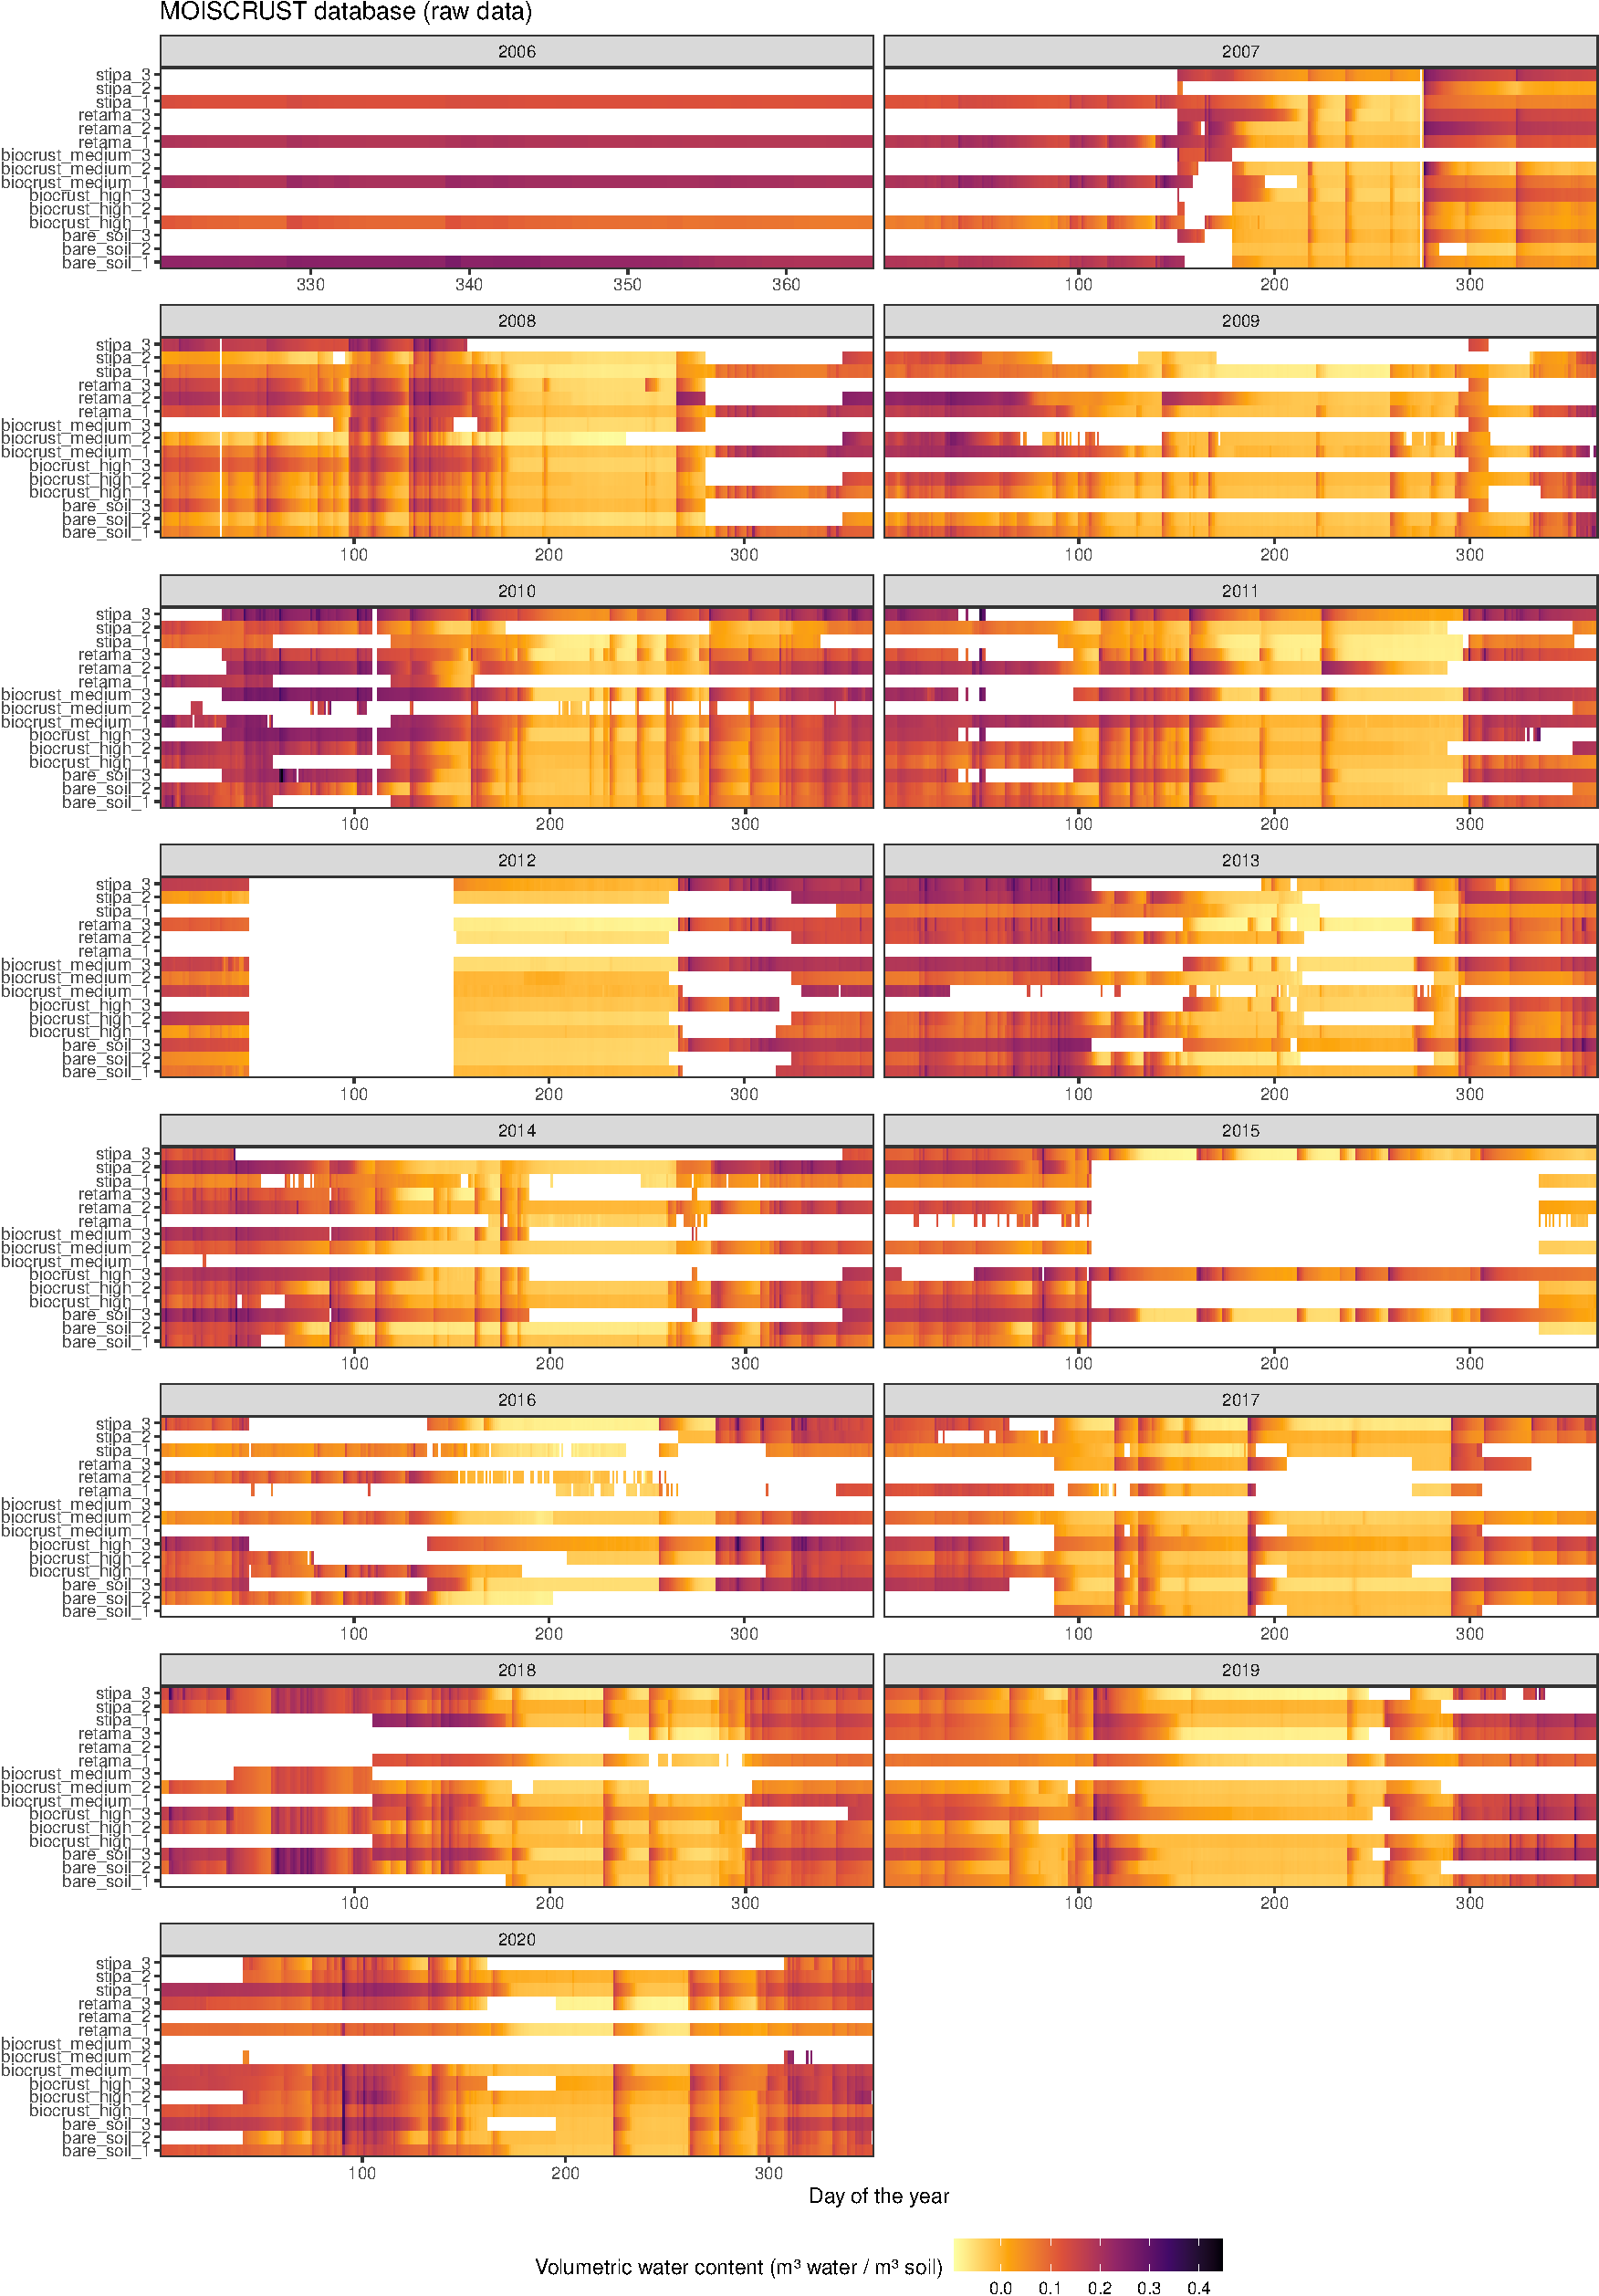
\includegraphics{moiscrust_files/figure-latex/unnamed-chunk-8-1.pdf}

\hypertarget{number-of-na-per-sensor}{%
\subsection{Number of NA per sensor}\label{number-of-na-per-sensor}}

Due to technical constraints, there is a large number of missing data in
the \emph{MOISCRUST} dataset. To better understand the extent of such
missing data, the code below counts the number of missing entries per
sensor.

\begin{Shaded}
\begin{Highlighting}[]
\CommentTok{#counting NA values per sensor}
\NormalTok{moiscrust_NA <-}\StringTok{ }\NormalTok{moiscrust_long }\OperatorTok\StringTok{ }
\StringTok{  }\KeywordTok{group_by}\NormalTok{(sensor) }\OperatorTok\StringTok{ }
\StringTok{  }\KeywordTok{summarise}\NormalTok{(}\DataTypeTok{na_count =} \KeywordTok{sum}\NormalTok{(}\KeywordTok{is.na}\NormalTok{(soil_moisture))) }\OperatorTok\StringTok{ }
\StringTok{  }\KeywordTok{mutate}\NormalTok{(}\DataTypeTok{na_count_percent =} \KeywordTok{round}\NormalTok{((na_count }\OperatorTok{*}\StringTok{ }\DecValTok{100}\NormalTok{) }\OperatorTok{/}\StringTok{ }\KeywordTok{nrow}\NormalTok{(moiscrust), }\DecValTok{1}\NormalTok{))}

\CommentTok{#adding sensor microsite to the moiscrust_NA data frame}
\NormalTok{moiscrust_NA}\OperatorTok{$}\NormalTok{microsite <-}\StringTok{ }\KeywordTok{c}\NormalTok{(}
  \StringTok{"bare_soil"}\NormalTok{,}
  \StringTok{"bare_soil"}\NormalTok{,}
  \StringTok{"bare_soil"}\NormalTok{,}
  \StringTok{"biocrust_high"}\NormalTok{,}
  \StringTok{"biocrust_high"}\NormalTok{,}
  \StringTok{"biocrust_high"}\NormalTok{,}
  \StringTok{"biocrust_medium"}\NormalTok{,}
  \StringTok{"biocrust_medium"}\NormalTok{,}
  \StringTok{"biocrust_medium"}\NormalTok{,}
  \StringTok{"retama"}\NormalTok{,}
  \StringTok{"retama"}\NormalTok{,}
  \StringTok{"retama"}\NormalTok{,}
  \StringTok{"stipa"}\NormalTok{,}
  \StringTok{"stipa"}\NormalTok{,}
  \StringTok{"stipa"}
\NormalTok{)}

\CommentTok{#reordering columns and arranging by na_count}
\NormalTok{moiscrust_NA <-}\StringTok{ }\NormalTok{moiscrust_NA[, }\KeywordTok{c}\NormalTok{(}
  \StringTok{"sensor"}\NormalTok{, }
  \StringTok{"microsite"}\NormalTok{, }
  \StringTok{"na_count"}\NormalTok{, }
  \StringTok{"na_count_percent"}
\NormalTok{  )] }\OperatorTok\StringTok{ }
\StringTok{  }\NormalTok{dplyr}\OperatorTok{::}\KeywordTok{arrange}\NormalTok{(na_count) }\OperatorTok\StringTok{ }
\StringTok{  }\KeywordTok{as.data.frame}\NormalTok{()}
\end{Highlighting}
\end{Shaded}

\begin{table}[H]
\centering
\begin{tabular}[t]{l|l|r|r}
\hline
sensor & microsite & na\_count & na\_count\_percent\\
\hline
\cellcolor{gray!6}{biocrust\_high\_1} & \cellcolor{gray!6}{biocrust\_high} & \cellcolor{gray!6}{7674} & \cellcolor{gray!6}{16.5}\\
\hline
stipa\_1 & stipa & 10553 & 22.7\\
\hline
\cellcolor{gray!6}{bare\_soil\_1} & \cellcolor{gray!6}{bare\_soil} & \cellcolor{gray!6}{10987} & \cellcolor{gray!6}{23.6}\\
\hline
bare\_soil\_3 & bare\_soil & 11114 & 23.9\\
\hline
\cellcolor{gray!6}{bare\_soil\_2} & \cellcolor{gray!6}{bare\_soil} & \cellcolor{gray!6}{11188} & \cellcolor{gray!6}{24.1}\\
\hline
biocrust\_high\_2 & biocrust\_high & 11776 & 25.3\\
\hline
\cellcolor{gray!6}{biocrust\_high\_3} & \cellcolor{gray!6}{biocrust\_high} & \cellcolor{gray!6}{14125} & \cellcolor{gray!6}{30.4}\\
\hline
stipa\_2 & stipa & 15363 & 33.0\\
\hline
\cellcolor{gray!6}{stipa\_3} & \cellcolor{gray!6}{stipa} & \cellcolor{gray!6}{15604} & \cellcolor{gray!6}{33.5}\\
\hline
biocrust\_medium\_1 & biocrust\_medium & 16934 & 36.4\\
\hline
\cellcolor{gray!6}{biocrust\_medium\_2} & \cellcolor{gray!6}{biocrust\_medium} & \cellcolor{gray!6}{18743} & \cellcolor{gray!6}{40.3}\\
\hline
retama\_3 & retama & 20505 & 44.1\\
\hline
\cellcolor{gray!6}{retama\_1} & \cellcolor{gray!6}{retama} & \cellcolor{gray!6}{22840} & \cellcolor{gray!6}{49.1}\\
\hline
retama\_2 & retama & 22999 & 49.4\\
\hline
\cellcolor{gray!6}{biocrust\_medium\_3} & \cellcolor{gray!6}{biocrust\_medium} & \cellcolor{gray!6}{31225} & \cellcolor{gray!6}{67.1}\\
\hline
\end{tabular}
\end{table}

\hypertarget{imputation-of-missing-data}{%
\section{Imputation of missing data}\label{imputation-of-missing-data}}

The imputation of missing data we implement here to impute missing data
in \emph{MOISCRUST} works by finding, for a given entry \emph{y} with
missing data at a time \emph{t}, the sensor \emph{x} with data for
\emph{t} that is in the same type of microsite (if possible), has the
longest extent in common, and the highest correlation with the sensor to
which \emph{y} belongs, and estimates \emph{y} with the linear model
\emph{y \textasciitilde{} x}.

\hypertarget{developing-criteria-to-find-candidates-for-gap-filling}{%
\subsection{Developing criteria to find candidates for gap
filling}\label{developing-criteria-to-find-candidates-for-gap-filling}}

To generate the criteria to find the best possible candidate \emph{x} to
estimate the missing data \emph{y}, we compute the common length and
correlation between all pairs of sensors, and generate a column
indicating whether they belong to the same microsite or not. With the
values stored in these columns we compute a \emph{selection score} based
on the following expression:

\[S_{x} = \%vc_{x, y} + (R_{x, y}^2 * 100) + \left\{
\begin{array}{ll}
      100, & \mbox{if $microsite_{x} == microsite_{y}$}\\
      0, & \mbox{otherwise}
\end{array}
\right. \]

Where:

\begin{itemize}
\tightlist
\item
  \(y\) is the sensor with a missing value to be estimated.
\item
  \(x\) is the sensor to be used as candidate predictor to estimate the
  missing value in \(y\).
\item
  \(S_{x}\) is the selection score of the candidate sensor \(x\), in the
  range {[}0, 300{]}.
\item
  \(\%vc_{x, y}\) is the percent of common valid cases of the sensors
  \(x\) and \(y\).
\item
  \(R_{x, y}^2\) is the Pearson's R² of the common valid cases of the
  sensors \(x\) and \(y\).
\item
  \(microsite_{x}\) and \(microsite_{y}\) are the respective microsites
  of the sensors \(x\) and \(y\).
\end{itemize}

During data imputation, for each missing value, the sensor with the
higher selection score is used to estimate it.

These criteria are stored in the data frame \textbf{sensors\_pairs}.
Along with the computation of the selection score, the code below also
computes a linear model for each pair \(x ~ y\), and stores it in the
object \textbf{sensors\_pairs\_models}. The identificators of these
models are stored in the column \emph{model\_id} of the data frame
\textbf{sensors\_pairs}.

\begin{Shaded}
\begin{Highlighting}[]
\CommentTok{#combining sensors in pairs x-y}
\NormalTok{sensors_pairs <-}\StringTok{ }\KeywordTok{combn}\NormalTok{(}
  \DataTypeTok{x =}\NormalTok{ sensors,}
  \DataTypeTok{m =} \DecValTok{2}
\NormalTok{) }\OperatorTok\StringTok{ }
\StringTok{  }\KeywordTok{t}\NormalTok{() }\OperatorTok\StringTok{ }
\StringTok{  }\KeywordTok{as.data.frame}\NormalTok{()}

\CommentTok{#adding combinations y-x so all pairs have both directions}
\CommentTok{#removing repeated pairs}
\CommentTok{#joining with moiscrust_NA to get sensor groups}
\CommentTok{#add column same_microsite to check if x and y are or not in the same sensor group}
\CommentTok{#add empty columns to store % of shared data, model's R squared, and model ID}
\NormalTok{sensors_pairs <-}\StringTok{ }\NormalTok{sensors_pairs }\OperatorTok\StringTok{ }
\StringTok{  }\KeywordTok{rbind}\NormalTok{(}
    \KeywordTok{data.frame}\NormalTok{(}
      \DataTypeTok{V1 =}\NormalTok{ sensors_pairs}\OperatorTok{$}\NormalTok{V2,}
      \DataTypeTok{V2 =}\NormalTok{ sensors_pairs}\OperatorTok{$}\NormalTok{V1}
\NormalTok{    )}
\NormalTok{  ) }\OperatorTok\StringTok{ }
\StringTok{  }\KeywordTok{distinct}\NormalTok{(}
\NormalTok{    V1, }
\NormalTok{    V2, }
    \DataTypeTok{.keep_all =} \OtherTok{TRUE}
\NormalTok{  ) }\OperatorTok\StringTok{ }
\StringTok{  }\KeywordTok{left_join}\NormalTok{(}
\NormalTok{    moiscrust_NA[, }\KeywordTok{c}\NormalTok{(}\StringTok{"sensor"}\NormalTok{, }\StringTok{"microsite"}\NormalTok{)],}
    \DataTypeTok{by =} \KeywordTok{c}\NormalTok{(}\StringTok{"V1"}\NormalTok{ =}\StringTok{ "sensor"}\NormalTok{)}
\NormalTok{  ) }\OperatorTok\StringTok{ }
\StringTok{  }\KeywordTok{left_join}\NormalTok{(}
\NormalTok{    moiscrust_NA[, }\KeywordTok{c}\NormalTok{(}\StringTok{"sensor"}\NormalTok{, }\StringTok{"microsite"}\NormalTok{)],}
    \DataTypeTok{by =} \KeywordTok{c}\NormalTok{(}\StringTok{"V2"}\NormalTok{ =}\StringTok{ "sensor"}\NormalTok{)}
\NormalTok{  ) }\OperatorTok\StringTok{ }
\StringTok{  }\KeywordTok{rename}\NormalTok{(}
    \DataTypeTok{y =}\NormalTok{ V1,}
    \DataTypeTok{x =}\NormalTok{ V2,}
    \DataTypeTok{y_microsite =}\NormalTok{ microsite.x, }\CommentTok{#not a mistake}
    \DataTypeTok{x_microsite =}\NormalTok{ microsite.y, }\CommentTok{#not a mistake}
\NormalTok{  ) }\OperatorTok\StringTok{ }
\StringTok{  }\KeywordTok{mutate}\NormalTok{(}
    \DataTypeTok{same_microsite =} \KeywordTok{ifelse}\NormalTok{(}
\NormalTok{      x_microsite }\OperatorTok{==}\StringTok{ }\NormalTok{y_microsite, }
      \OtherTok{TRUE}\NormalTok{, }
      \OtherTok{FALSE}
\NormalTok{      ),}
    \DataTypeTok{sensors_shared_valid_percent =} \OtherTok{NA}\NormalTok{,}
    \DataTypeTok{sensors_r_squared =} \OtherTok{NA}\NormalTok{,}
    \DataTypeTok{model_id =} \KeywordTok{row_number}\NormalTok{()}
\NormalTok{  ) }

\CommentTok{#list to store models}
\NormalTok{sensors_pairs_models <-}\StringTok{ }\KeywordTok{list}\NormalTok{()}

\CommentTok{#looping through sensors pairs to:}
\CommentTok{#fit lm model y ~ x and save it in sensors_pairs_models}
\CommentTok{#}
\ControlFlowTok{for}\NormalTok{(i }\ControlFlowTok{in} \DecValTok{1}\OperatorTok{:}\KeywordTok{nrow}\NormalTok{(sensors_pairs))\{}
  
  \CommentTok{#names of the sensors y and x}
\NormalTok{  y_i <-}\StringTok{ }\NormalTok{sensors_pairs[i, }\StringTok{"y"}\NormalTok{]}
\NormalTok{  x_i <-}\StringTok{ }\NormalTok{sensors_pairs[i, }\StringTok{"x"}\NormalTok{]}
  
  \CommentTok{#data of the sensor pair}
\NormalTok{  sensor_pair_i <-}\StringTok{ }\NormalTok{moiscrust[, }\KeywordTok{c}\NormalTok{(y_i, x_i)]}
  
  \CommentTok{#complete cases of the sensor pair}
\NormalTok{  sensor_pair_i <-}\StringTok{ }\NormalTok{sensor_pair_i[}\KeywordTok{complete.cases}\NormalTok{(sensor_pair_i), ]}
   
  \CommentTok{#common cases}
\NormalTok{  sensors_pairs[i, }\StringTok{"sensors_shared_valid_percent"}\NormalTok{] <-}\StringTok{ }
\StringTok{    }\KeywordTok{nrow}\NormalTok{(sensor_pair_i) }\OperatorTok{/}\StringTok{ }\KeywordTok{nrow}\NormalTok{(moiscrust) }\OperatorTok{*}\StringTok{ }\DecValTok{100}
  
  \CommentTok{#R squared of the sensor pair}
\NormalTok{  sensors_pairs[i, }\StringTok{"sensors_r_squared"}\NormalTok{] <-}\StringTok{ }\KeywordTok{cor}\NormalTok{(}
\NormalTok{    sensor_pair_i[, }\DecValTok{1}\NormalTok{],}
\NormalTok{    sensor_pair_i[, }\DecValTok{2}\NormalTok{]}
\NormalTok{    )}
  
  \CommentTok{#model formula y ~ x}
\NormalTok{  formula_i <-}\StringTok{ }\KeywordTok{as.formula}\NormalTok{(}\KeywordTok{paste}\NormalTok{(y_i, }\StringTok{"~"}\NormalTok{, x_i))}
  
  \CommentTok{#linear model}
\NormalTok{  sensors_pairs_models[[i]] <-}\StringTok{ }\KeywordTok{lm}\NormalTok{(}
    \DataTypeTok{formula =}\NormalTok{ formula_i,}
    \DataTypeTok{data =}\NormalTok{ sensor_pair_i}
\NormalTok{  )}
  
\NormalTok{\}}

\CommentTok{#selection score to find candidates during gap filling }
\CommentTok{#(sensors_r_squared * 100) +}
\CommentTok{#sensors_shared_valid_percent + }
\CommentTok{#same_microsite (TRUE = 100, FALSE = 0)}
\NormalTok{sensors_pairs <-}\StringTok{ }\KeywordTok{mutate}\NormalTok{(}
\NormalTok{  sensors_pairs,}
  \DataTypeTok{selection_score =} 
\NormalTok{    (sensors_r_squared }\OperatorTok{*}\StringTok{ }\DecValTok{100}\NormalTok{) }\OperatorTok{+}\StringTok{ }
\StringTok{    }\NormalTok{sensors_shared_valid_percent }\OperatorTok{+}\StringTok{ }
\StringTok{    }\KeywordTok{ifelse}\NormalTok{(same_microsite }\OperatorTok{==}\StringTok{ }\OtherTok{TRUE}\NormalTok{, }\DecValTok{100}\NormalTok{, }\DecValTok{0}\NormalTok{)}
\NormalTok{)}

\CommentTok{#removing objects we don't need}
\KeywordTok{rm}\NormalTok{(}
\NormalTok{  sensor_pair_i,}
\NormalTok{  formula_i,}
\NormalTok{  i,}
\NormalTok{  x_i,}
\NormalTok{  y_i}
\NormalTok{)}
\end{Highlighting}
\end{Shaded}

The resulting data frame, named \textbf{sensors\_pairs}, has columns
with the names of the sensor \emph{y} (the one with missing data to
impute), the sensor \emph{x} (the candidate to be used as predictor to
estimate \emph{y}), their respective microsites, a column indicating if
they belong to the same microsite, the percent of shared valid data, the
R squared of their shared data, a

\begin{table}[H]
\centering
\resizebox{\linewidth}{!}{
\begin{tabular}[t]{l|l|l|l|l|r|r|r|r}
\hline
y & x & y\_microsite & x\_microsite & same\_microsite & sensors\_shared\_valid\_percent & sensors\_r\_squared & model\_id & selection\_score\\
\hline
\cellcolor{gray!6}{retama\_1} & \cellcolor{gray!6}{retama\_2} & \cellcolor{gray!6}{retama} & \cellcolor{gray!6}{retama} & \cellcolor{gray!6}{TRUE} & \cellcolor{gray!6}{20.503945} & \cellcolor{gray!6}{0.8825786} & \cellcolor{gray!6}{1} & \cellcolor{gray!6}{208.76181}\\
\hline
retama\_1 & retama\_3 & retama & retama & TRUE & 28.736052 & 0.9065618 & 2 & 219.39223\\
\hline
\cellcolor{gray!6}{retama\_1} & \cellcolor{gray!6}{stipa\_1} & \cellcolor{gray!6}{retama} & \cellcolor{gray!6}{stipa} & \cellcolor{gray!6}{FALSE} & \cellcolor{gray!6}{49.437792} & \cellcolor{gray!6}{0.6546707} & \cellcolor{gray!6}{3} & \cellcolor{gray!6}{114.90486}\\
\hline
retama\_1 & stipa\_2 & retama & stipa & FALSE & 34.751575 & 0.6570769 & 4 & 100.45926\\
\hline
\cellcolor{gray!6}{retama\_1} & \cellcolor{gray!6}{stipa\_3} & \cellcolor{gray!6}{retama} & \cellcolor{gray!6}{stipa} & \cellcolor{gray!6}{FALSE} & \cellcolor{gray!6}{27.985724} & \cellcolor{gray!6}{0.8494829} & \cellcolor{gray!6}{5} & \cellcolor{gray!6}{112.93401}\\
\hline
retama\_1 & bare\_soil\_1 & retama & bare\_soil & FALSE & 45.825898 & 0.8610431 & 6 & 131.93021\\
\hline
\cellcolor{gray!6}{retama\_1} & \cellcolor{gray!6}{bare\_soil\_2} & \cellcolor{gray!6}{retama} & \cellcolor{gray!6}{bare\_soil} & \cellcolor{gray!6}{FALSE} & \cellcolor{gray!6}{39.137445} & \cellcolor{gray!6}{0.6276224} & \cellcolor{gray!6}{7} & \cellcolor{gray!6}{101.89968}\\
\hline
retama\_1 & bare\_soil\_3 & retama & bare\_soil & FALSE & 34.364586 & 0.8118848 & 8 & 115.55307\\
\hline
\cellcolor{gray!6}{retama\_1} & \cellcolor{gray!6}{biocrust\_medium\_1} & \cellcolor{gray!6}{retama} & \cellcolor{gray!6}{biocrust\_medium} & \cellcolor{gray!6}{FALSE} & \cellcolor{gray!6}{44.099499} & \cellcolor{gray!6}{0.8808309} & \cellcolor{gray!6}{9} & \cellcolor{gray!6}{132.18258}\\
\hline
retama\_1 & biocrust\_medium\_2 & retama & biocrust\_medium & FALSE & 31.105282 & 0.7429876 & 10 & 105.40404\\
\hline
\cellcolor{gray!6}{retama\_1} & \cellcolor{gray!6}{biocrust\_medium\_3} & \cellcolor{gray!6}{retama} & \cellcolor{gray!6}{biocrust\_medium} & \cellcolor{gray!6}{FALSE} & \cellcolor{gray!6}{5.892976} & \cellcolor{gray!6}{0.8384753} & \cellcolor{gray!6}{11} & \cellcolor{gray!6}{89.74050}\\
\hline
retama\_1 & biocrust\_high\_1 & retama & biocrust\_high & FALSE & 48.414422 & 0.7630192 & 12 & 124.71634\\
\hline
\cellcolor{gray!6}{retama\_1} & \cellcolor{gray!6}{biocrust\_high\_2} & \cellcolor{gray!6}{retama} & \cellcolor{gray!6}{biocrust\_high} & \cellcolor{gray!6}{FALSE} & \cellcolor{gray!6}{38.305420} & \cellcolor{gray!6}{0.7500951} & \cellcolor{gray!6}{13} & \cellcolor{gray!6}{113.31493}\\
\hline
retama\_1 & biocrust\_high\_3 & retama & biocrust\_high & FALSE & 32.943478 & 0.8490180 & 14 & 117.84528\\
\hline
\cellcolor{gray!6}{retama\_2} & \cellcolor{gray!6}{retama\_3} & \cellcolor{gray!6}{retama} & \cellcolor{gray!6}{retama} & \cellcolor{gray!6}{TRUE} & \cellcolor{gray!6}{32.057704} & \cellcolor{gray!6}{0.8394976} & \cellcolor{gray!6}{15} & \cellcolor{gray!6}{216.00746}\\
\hline
retama\_2 & stipa\_1 & retama & stipa & FALSE & 42.633242 & 0.7653060 & 16 & 119.16384\\
\hline
\cellcolor{gray!6}{retama\_2} & \cellcolor{gray!6}{stipa\_2} & \cellcolor{gray!6}{retama} & \cellcolor{gray!6}{stipa} & \cellcolor{gray!6}{FALSE} & \cellcolor{gray!6}{37.522843} & \cellcolor{gray!6}{0.5339814} & \cellcolor{gray!6}{17} & \cellcolor{gray!6}{90.92099}\\
\hline
retama\_2 & stipa\_3 & retama & stipa & FALSE & 31.636317 & 0.8561540 & 18 & 117.25171\\
\hline
\cellcolor{gray!6}{retama\_2} & \cellcolor{gray!6}{bare\_soil\_1} & \cellcolor{gray!6}{retama} & \cellcolor{gray!6}{bare\_soil} & \cellcolor{gray!6}{FALSE} & \cellcolor{gray!6}{43.684561} & \cellcolor{gray!6}{0.7455036} & \cellcolor{gray!6}{19} & \cellcolor{gray!6}{118.23492}\\
\hline
retama\_2 & bare\_soil\_2 & retama & bare\_soil & FALSE & 48.896008 & 0.6940089 & 20 & 118.29689\\
\hline
\end{tabular}}
\end{table}

\hypertarget{generating-the-x-and-y-matrices-to-predict-imputed-values}{%
\subsection{Generating the x and y matrices to predict imputed
values}\label{generating-the-x-and-y-matrices-to-predict-imputed-values}}

During data imputation, two data frames are needed. The data frame
\textbf{x} contains the data of every sensor for every available time,
while the data frame \textbf{y}, which starts with empty values, is
where the imputed values, their confidence intervals, selection
criteria, and other quality-related columns are going to be stored.

\begin{Shaded}
\begin{Highlighting}[]
\CommentTok{#creating data frame of predictors}
\NormalTok{x <-}\StringTok{ }\NormalTok{moiscrust[, sensors]}

\CommentTok{#creating data frame to store model results}
\NormalTok{y <-}\StringTok{ }\KeywordTok{matrix}\NormalTok{(}
  \DataTypeTok{data =} \OtherTok{NA}\NormalTok{, }
  \DataTypeTok{nrow =} \KeywordTok{nrow}\NormalTok{(moiscrust), }
  \DataTypeTok{ncol =} \DecValTok{12}
\NormalTok{  ) }\OperatorTok\StringTok{ }
\StringTok{  }\KeywordTok{as.data.frame}\NormalTok{()}

\CommentTok{#new colnames}
\KeywordTok{colnames}\NormalTok{(y) <-}\StringTok{ }\KeywordTok{c}\NormalTok{(}
  \StringTok{"interpolated"}\NormalTok{,}
  \StringTok{"model_estimate"}\NormalTok{, }
  \StringTok{"model_ci_lower"}\NormalTok{, }
  \StringTok{"model_ci_upper"}\NormalTok{, }
  \StringTok{"model_predictor"}\NormalTok{,}
  \StringTok{"same_microsite"}\NormalTok{,}
  \StringTok{"sensors_r_squared"}\NormalTok{,}
  \StringTok{"sensors_shared_valid_percent"}\NormalTok{,}
  \StringTok{"selection_score"}\NormalTok{,}
  \StringTok{"date_time_id"}\NormalTok{,}
  \StringTok{"sensor"}\NormalTok{,}
  \StringTok{"microsite"}
\NormalTok{  )}

\CommentTok{#transferring time id}
\NormalTok{y[, }\StringTok{"date_time_id"}\NormalTok{] <-}\StringTok{ }\NormalTok{moiscrust[, }\StringTok{"date_time_id"}\NormalTok{]}
\NormalTok{y[, }\StringTok{"interpolated"}\NormalTok{] <-}\StringTok{ }\OtherTok{FALSE}
\end{Highlighting}
\end{Shaded}

The \textbf{x} data frame looks as follows:

\begin{table}[H]
\centering
\resizebox{\linewidth}{!}{
\begin{tabular}[t]{r|r|r|r|r|r|r|r|r|r|r|r|r|r|r}
\hline
retama\_1 & retama\_2 & retama\_3 & stipa\_1 & stipa\_2 & stipa\_3 & bare\_soil\_1 & bare\_soil\_2 & bare\_soil\_3 & biocrust\_medium\_1 & biocrust\_medium\_2 & biocrust\_medium\_3 & biocrust\_high\_1 & biocrust\_high\_2 & biocrust\_high\_3\\
\hline
\cellcolor{gray!6}{0.197} & \cellcolor{gray!6}{NA} & \cellcolor{gray!6}{NA} & \cellcolor{gray!6}{0.132} & \cellcolor{gray!6}{NA} & \cellcolor{gray!6}{NA} & \cellcolor{gray!6}{0.232} & \cellcolor{gray!6}{NA} & \cellcolor{gray!6}{NA} & \cellcolor{gray!6}{0.205} & \cellcolor{gray!6}{NA} & \cellcolor{gray!6}{NA} & \cellcolor{gray!6}{0.121} & \cellcolor{gray!6}{NA} & \cellcolor{gray!6}{NA}\\
\hline
0.195 & NA & NA & 0.131 & NA & NA & 0.233 & NA & NA & 0.203 & NA & NA & 0.117 & NA & NA\\
\hline
\cellcolor{gray!6}{0.194} & \cellcolor{gray!6}{NA} & \cellcolor{gray!6}{NA} & \cellcolor{gray!6}{0.131} & \cellcolor{gray!6}{NA} & \cellcolor{gray!6}{NA} & \cellcolor{gray!6}{0.234} & \cellcolor{gray!6}{NA} & \cellcolor{gray!6}{NA} & \cellcolor{gray!6}{0.203} & \cellcolor{gray!6}{NA} & \cellcolor{gray!6}{NA} & \cellcolor{gray!6}{0.117} & \cellcolor{gray!6}{NA} & \cellcolor{gray!6}{NA}\\
\hline
0.194 & NA & NA & 0.131 & NA & NA & 0.234 & NA & NA & 0.203 & NA & NA & 0.116 & NA & NA\\
\hline
\cellcolor{gray!6}{0.194} & \cellcolor{gray!6}{NA} & \cellcolor{gray!6}{NA} & \cellcolor{gray!6}{0.130} & \cellcolor{gray!6}{NA} & \cellcolor{gray!6}{NA} & \cellcolor{gray!6}{0.234} & \cellcolor{gray!6}{NA} & \cellcolor{gray!6}{NA} & \cellcolor{gray!6}{0.203} & \cellcolor{gray!6}{NA} & \cellcolor{gray!6}{NA} & \cellcolor{gray!6}{0.116} & \cellcolor{gray!6}{NA} & \cellcolor{gray!6}{NA}\\
\hline
0.194 & NA & NA & 0.130 & NA & NA & 0.234 & NA & NA & 0.202 & NA & NA & 0.116 & NA & \vphantom{1} NA\\
\hline
\cellcolor{gray!6}{0.194} & \cellcolor{gray!6}{NA} & \cellcolor{gray!6}{NA} & \cellcolor{gray!6}{0.130} & \cellcolor{gray!6}{NA} & \cellcolor{gray!6}{NA} & \cellcolor{gray!6}{0.234} & \cellcolor{gray!6}{NA} & \cellcolor{gray!6}{NA} & \cellcolor{gray!6}{0.202} & \cellcolor{gray!6}{NA} & \cellcolor{gray!6}{NA} & \cellcolor{gray!6}{0.115} & \cellcolor{gray!6}{NA} & \cellcolor{gray!6}{\vphantom{2} NA}\\
\hline
0.194 & NA & NA & 0.130 & NA & NA & 0.234 & NA & NA & 0.202 & NA & NA & 0.115 & NA & \vphantom{1} NA\\
\hline
\cellcolor{gray!6}{0.194} & \cellcolor{gray!6}{NA} & \cellcolor{gray!6}{NA} & \cellcolor{gray!6}{0.130} & \cellcolor{gray!6}{NA} & \cellcolor{gray!6}{NA} & \cellcolor{gray!6}{0.234} & \cellcolor{gray!6}{NA} & \cellcolor{gray!6}{NA} & \cellcolor{gray!6}{0.202} & \cellcolor{gray!6}{NA} & \cellcolor{gray!6}{NA} & \cellcolor{gray!6}{0.115} & \cellcolor{gray!6}{NA} & \cellcolor{gray!6}{NA}\\
\hline
0.194 & NA & NA & 0.130 & NA & NA & 0.234 & NA & NA & 0.202 & NA & NA & 0.116 & NA & NA\\
\hline
\cellcolor{gray!6}{0.195} & \cellcolor{gray!6}{NA} & \cellcolor{gray!6}{NA} & \cellcolor{gray!6}{0.131} & \cellcolor{gray!6}{NA} & \cellcolor{gray!6}{NA} & \cellcolor{gray!6}{0.234} & \cellcolor{gray!6}{NA} & \cellcolor{gray!6}{NA} & \cellcolor{gray!6}{0.202} & \cellcolor{gray!6}{NA} & \cellcolor{gray!6}{NA} & \cellcolor{gray!6}{0.116} & \cellcolor{gray!6}{NA} & \cellcolor{gray!6}{NA}\\
\hline
0.195 & NA & NA & 0.131 & NA & NA & 0.233 & NA & NA & 0.201 & NA & NA & 0.115 & NA & NA\\
\hline
\cellcolor{gray!6}{0.194} & \cellcolor{gray!6}{NA} & \cellcolor{gray!6}{NA} & \cellcolor{gray!6}{0.130} & \cellcolor{gray!6}{NA} & \cellcolor{gray!6}{NA} & \cellcolor{gray!6}{0.233} & \cellcolor{gray!6}{NA} & \cellcolor{gray!6}{NA} & \cellcolor{gray!6}{0.200} & \cellcolor{gray!6}{NA} & \cellcolor{gray!6}{NA} & \cellcolor{gray!6}{0.114} & \cellcolor{gray!6}{NA} & \cellcolor{gray!6}{NA}\\
\hline
0.193 & NA & NA & 0.129 & NA & NA & 0.233 & NA & NA & 0.199 & NA & NA & 0.112 & NA & NA\\
\hline
\cellcolor{gray!6}{0.192} & \cellcolor{gray!6}{NA} & \cellcolor{gray!6}{NA} & \cellcolor{gray!6}{0.129} & \cellcolor{gray!6}{NA} & \cellcolor{gray!6}{NA} & \cellcolor{gray!6}{0.234} & \cellcolor{gray!6}{NA} & \cellcolor{gray!6}{NA} & \cellcolor{gray!6}{0.199} & \cellcolor{gray!6}{NA} & \cellcolor{gray!6}{NA} & \cellcolor{gray!6}{0.111} & \cellcolor{gray!6}{NA} & \cellcolor{gray!6}{NA}\\
\hline
0.192 & NA & NA & 0.128 & NA & NA & 0.234 & NA & NA & 0.199 & NA & NA & 0.111 & NA & NA\\
\hline
\cellcolor{gray!6}{0.191} & \cellcolor{gray!6}{NA} & \cellcolor{gray!6}{NA} & \cellcolor{gray!6}{0.128} & \cellcolor{gray!6}{NA} & \cellcolor{gray!6}{NA} & \cellcolor{gray!6}{0.234} & \cellcolor{gray!6}{NA} & \cellcolor{gray!6}{NA} & \cellcolor{gray!6}{0.198} & \cellcolor{gray!6}{NA} & \cellcolor{gray!6}{NA} & \cellcolor{gray!6}{0.110} & \cellcolor{gray!6}{NA} & \cellcolor{gray!6}{NA}\\
\hline
0.190 & NA & NA & 0.127 & NA & NA & 0.234 & NA & NA & 0.198 & NA & NA & 0.109 & NA & NA\\
\hline
\cellcolor{gray!6}{0.189} & \cellcolor{gray!6}{NA} & \cellcolor{gray!6}{NA} & \cellcolor{gray!6}{0.127} & \cellcolor{gray!6}{NA} & \cellcolor{gray!6}{NA} & \cellcolor{gray!6}{0.234} & \cellcolor{gray!6}{NA} & \cellcolor{gray!6}{NA} & \cellcolor{gray!6}{0.198} & \cellcolor{gray!6}{NA} & \cellcolor{gray!6}{NA} & \cellcolor{gray!6}{0.109} & \cellcolor{gray!6}{NA} & \cellcolor{gray!6}{NA}\\
\hline
0.188 & NA & NA & 0.127 & NA & NA & 0.234 & NA & NA & 0.198 & NA & NA & 0.109 & NA & NA\\
\hline
\end{tabular}}
\end{table}

And this is the \textbf{y} data frame, that will be filled during data
imputation:

\begin{table}[H]
\centering
\resizebox{\linewidth}{!}{
\begin{tabular}[t]{l|l|l|l|l|l|l|l|l|r|l|l}
\hline
interpolated & model\_estimate & model\_ci\_lower & model\_ci\_upper & model\_predictor & same\_microsite & sensors\_r\_squared & sensors\_shared\_valid\_percent & selection\_score & date\_time\_id & sensor & microsite\\
\hline
\cellcolor{gray!6}{FALSE} & \cellcolor{gray!6}{NA} & \cellcolor{gray!6}{NA} & \cellcolor{gray!6}{NA} & \cellcolor{gray!6}{NA} & \cellcolor{gray!6}{NA} & \cellcolor{gray!6}{NA} & \cellcolor{gray!6}{NA} & \cellcolor{gray!6}{NA} & \cellcolor{gray!6}{1} & \cellcolor{gray!6}{NA} & \cellcolor{gray!6}{NA}\\
\hline
FALSE & NA & NA & NA & NA & NA & NA & NA & NA & 2 & NA & NA\\
\hline
\cellcolor{gray!6}{FALSE} & \cellcolor{gray!6}{NA} & \cellcolor{gray!6}{NA} & \cellcolor{gray!6}{NA} & \cellcolor{gray!6}{NA} & \cellcolor{gray!6}{NA} & \cellcolor{gray!6}{NA} & \cellcolor{gray!6}{NA} & \cellcolor{gray!6}{NA} & \cellcolor{gray!6}{3} & \cellcolor{gray!6}{NA} & \cellcolor{gray!6}{NA}\\
\hline
FALSE & NA & NA & NA & NA & NA & NA & NA & NA & 4 & NA & NA\\
\hline
\cellcolor{gray!6}{FALSE} & \cellcolor{gray!6}{NA} & \cellcolor{gray!6}{NA} & \cellcolor{gray!6}{NA} & \cellcolor{gray!6}{NA} & \cellcolor{gray!6}{NA} & \cellcolor{gray!6}{NA} & \cellcolor{gray!6}{NA} & \cellcolor{gray!6}{NA} & \cellcolor{gray!6}{5} & \cellcolor{gray!6}{NA} & \cellcolor{gray!6}{NA}\\
\hline
FALSE & NA & NA & NA & NA & NA & NA & NA & NA & 6 & NA & NA\\
\hline
\cellcolor{gray!6}{FALSE} & \cellcolor{gray!6}{NA} & \cellcolor{gray!6}{NA} & \cellcolor{gray!6}{NA} & \cellcolor{gray!6}{NA} & \cellcolor{gray!6}{NA} & \cellcolor{gray!6}{NA} & \cellcolor{gray!6}{NA} & \cellcolor{gray!6}{NA} & \cellcolor{gray!6}{7} & \cellcolor{gray!6}{NA} & \cellcolor{gray!6}{NA}\\
\hline
FALSE & NA & NA & NA & NA & NA & NA & NA & NA & 8 & NA & NA\\
\hline
\cellcolor{gray!6}{FALSE} & \cellcolor{gray!6}{NA} & \cellcolor{gray!6}{NA} & \cellcolor{gray!6}{NA} & \cellcolor{gray!6}{NA} & \cellcolor{gray!6}{NA} & \cellcolor{gray!6}{NA} & \cellcolor{gray!6}{NA} & \cellcolor{gray!6}{NA} & \cellcolor{gray!6}{9} & \cellcolor{gray!6}{NA} & \cellcolor{gray!6}{NA}\\
\hline
FALSE & NA & NA & NA & NA & NA & NA & NA & NA & 10 & NA & NA\\
\hline
\cellcolor{gray!6}{FALSE} & \cellcolor{gray!6}{NA} & \cellcolor{gray!6}{NA} & \cellcolor{gray!6}{NA} & \cellcolor{gray!6}{NA} & \cellcolor{gray!6}{NA} & \cellcolor{gray!6}{NA} & \cellcolor{gray!6}{NA} & \cellcolor{gray!6}{NA} & \cellcolor{gray!6}{11} & \cellcolor{gray!6}{NA} & \cellcolor{gray!6}{NA}\\
\hline
FALSE & NA & NA & NA & NA & NA & NA & NA & NA & 12 & NA & NA\\
\hline
\cellcolor{gray!6}{FALSE} & \cellcolor{gray!6}{NA} & \cellcolor{gray!6}{NA} & \cellcolor{gray!6}{NA} & \cellcolor{gray!6}{NA} & \cellcolor{gray!6}{NA} & \cellcolor{gray!6}{NA} & \cellcolor{gray!6}{NA} & \cellcolor{gray!6}{NA} & \cellcolor{gray!6}{13} & \cellcolor{gray!6}{NA} & \cellcolor{gray!6}{NA}\\
\hline
FALSE & NA & NA & NA & NA & NA & NA & NA & NA & 14 & NA & NA\\
\hline
\cellcolor{gray!6}{FALSE} & \cellcolor{gray!6}{NA} & \cellcolor{gray!6}{NA} & \cellcolor{gray!6}{NA} & \cellcolor{gray!6}{NA} & \cellcolor{gray!6}{NA} & \cellcolor{gray!6}{NA} & \cellcolor{gray!6}{NA} & \cellcolor{gray!6}{NA} & \cellcolor{gray!6}{15} & \cellcolor{gray!6}{NA} & \cellcolor{gray!6}{NA}\\
\hline
FALSE & NA & NA & NA & NA & NA & NA & NA & NA & 16 & NA & NA\\
\hline
\cellcolor{gray!6}{FALSE} & \cellcolor{gray!6}{NA} & \cellcolor{gray!6}{NA} & \cellcolor{gray!6}{NA} & \cellcolor{gray!6}{NA} & \cellcolor{gray!6}{NA} & \cellcolor{gray!6}{NA} & \cellcolor{gray!6}{NA} & \cellcolor{gray!6}{NA} & \cellcolor{gray!6}{17} & \cellcolor{gray!6}{NA} & \cellcolor{gray!6}{NA}\\
\hline
FALSE & NA & NA & NA & NA & NA & NA & NA & NA & 18 & NA & NA\\
\hline
\cellcolor{gray!6}{FALSE} & \cellcolor{gray!6}{NA} & \cellcolor{gray!6}{NA} & \cellcolor{gray!6}{NA} & \cellcolor{gray!6}{NA} & \cellcolor{gray!6}{NA} & \cellcolor{gray!6}{NA} & \cellcolor{gray!6}{NA} & \cellcolor{gray!6}{NA} & \cellcolor{gray!6}{19} & \cellcolor{gray!6}{NA} & \cellcolor{gray!6}{NA}\\
\hline
FALSE & NA & NA & NA & NA & NA & NA & NA & NA & 20 & NA & NA\\
\hline
\end{tabular}}
\end{table}

\hypertarget{data-imputation-step-by-step}{%
\subsection{Data imputation, step by
step}\label{data-imputation-step-by-step}}

The steps to fill the gaps in the \textbf{MOISCRUST} database go as
follows:

\textbf{1.} A given sensor name is selected: ``retama\_2''

\begin{Shaded}
\begin{Highlighting}[]
\NormalTok{sensor =}\StringTok{ "retama_2"}
\end{Highlighting}
\end{Shaded}

\textbf{2.} The sensors pairs from the table \textbf{sensors\_pairs}
where the selected sensor is \emph{y} (the sensor which values are to be
imputed) are selected.

\begin{Shaded}
\begin{Highlighting}[]
\NormalTok{sensors_pair <-}\StringTok{ }\NormalTok{sensors_pairs }\OperatorTok\StringTok{ }
\StringTok{    }\NormalTok{dplyr}\OperatorTok{::}\KeywordTok{filter}\NormalTok{(y }\OperatorTok{==}\StringTok{ }\NormalTok{sensor)}
\end{Highlighting}
\end{Shaded}

\begin{table}[H]
\centering
\resizebox{\linewidth}{!}{
\begin{tabular}[t]{l|l|l|l|l|r|r|r|r}
\hline
y & x & y\_microsite & x\_microsite & same\_microsite & sensors\_shared\_valid\_percent & sensors\_r\_squared & model\_id & selection\_score\\
\hline
\cellcolor{gray!6}{retama\_2} & \cellcolor{gray!6}{retama\_3} & \cellcolor{gray!6}{retama} & \cellcolor{gray!6}{retama} & \cellcolor{gray!6}{TRUE} & \cellcolor{gray!6}{32.05770} & \cellcolor{gray!6}{0.8394976} & \cellcolor{gray!6}{15} & \cellcolor{gray!6}{216.00746}\\
\hline
retama\_2 & stipa\_1 & retama & stipa & FALSE & 42.63324 & 0.7653060 & 16 & 119.16384\\
\hline
\cellcolor{gray!6}{retama\_2} & \cellcolor{gray!6}{stipa\_2} & \cellcolor{gray!6}{retama} & \cellcolor{gray!6}{stipa} & \cellcolor{gray!6}{FALSE} & \cellcolor{gray!6}{37.52284} & \cellcolor{gray!6}{0.5339814} & \cellcolor{gray!6}{17} & \cellcolor{gray!6}{90.92099}\\
\hline
retama\_2 & stipa\_3 & retama & stipa & FALSE & 31.63632 & 0.8561540 & 18 & 117.25171\\
\hline
\cellcolor{gray!6}{retama\_2} & \cellcolor{gray!6}{bare\_soil\_1} & \cellcolor{gray!6}{retama} & \cellcolor{gray!6}{bare\_soil} & \cellcolor{gray!6}{FALSE} & \cellcolor{gray!6}{43.68456} & \cellcolor{gray!6}{0.7455036} & \cellcolor{gray!6}{19} & \cellcolor{gray!6}{118.23492}\\
\hline
retama\_2 & bare\_soil\_2 & retama & bare\_soil & FALSE & 48.89601 & 0.6940089 & 20 & 118.29689\\
\hline
\cellcolor{gray!6}{retama\_2} & \cellcolor{gray!6}{bare\_soil\_3} & \cellcolor{gray!6}{retama} & \cellcolor{gray!6}{bare\_soil} & \cellcolor{gray!6}{FALSE} & \cellcolor{gray!6}{37.40030} & \cellcolor{gray!6}{0.7494452} & \cellcolor{gray!6}{21} & \cellcolor{gray!6}{112.34481}\\
\hline
retama\_2 & biocrust\_medium\_1 & retama & biocrust\_medium & FALSE & 30.22811 & 0.7692882 & 22 & 107.15692\\
\hline
\cellcolor{gray!6}{retama\_2} & \cellcolor{gray!6}{biocrust\_medium\_2} & \cellcolor{gray!6}{retama} & \cellcolor{gray!6}{biocrust\_medium} & \cellcolor{gray!6}{FALSE} & \cellcolor{gray!6}{37.38525} & \cellcolor{gray!6}{0.7255941} & \cellcolor{gray!6}{23} & \cellcolor{gray!6}{109.94466}\\
\hline
retama\_2 & biocrust\_medium\_3 & retama & biocrust\_medium & FALSE & 26.50872 & 0.8334687 & 24 & 109.85559\\
\hline
\cellcolor{gray!6}{retama\_2} & \cellcolor{gray!6}{biocrust\_high\_1} & \cellcolor{gray!6}{retama} & \cellcolor{gray!6}{biocrust\_high} & \cellcolor{gray!6}{FALSE} & \cellcolor{gray!6}{47.95649} & \cellcolor{gray!6}{0.6954543} & \cellcolor{gray!6}{25} & \cellcolor{gray!6}{117.50191}\\
\hline
retama\_2 & biocrust\_high\_2 & retama & biocrust\_high & FALSE & 47.88339 & 0.8146773 & 26 & 129.35112\\
\hline
\cellcolor{gray!6}{retama\_2} & \cellcolor{gray!6}{biocrust\_high\_3} & \cellcolor{gray!6}{retama} & \cellcolor{gray!6}{biocrust\_high} & \cellcolor{gray!6}{FALSE} & \cellcolor{gray!6}{33.64221} & \cellcolor{gray!6}{0.8001904} & \cellcolor{gray!6}{27} & \cellcolor{gray!6}{113.66124}\\
\hline
retama\_2 & retama\_1 & retama & retama & TRUE & 20.50395 & 0.8825786 & 106 & 208.76181\\
\hline
\end{tabular}}
\end{table}

\textbf{3.} The first row of the data frame \textbf{x} is selected.

\begin{Shaded}
\begin{Highlighting}[]
\NormalTok{x_row <-}\StringTok{ }\NormalTok{x[}\DecValTok{1}\NormalTok{, ]}
\end{Highlighting}
\end{Shaded}

\begin{table}[H]
\centering
\resizebox{\linewidth}{!}{
\begin{tabular}[t]{r|r|r|r|r|r|r|r|r|r|r|r|r|r|r}
\hline
retama\_1 & retama\_2 & retama\_3 & stipa\_1 & stipa\_2 & stipa\_3 & bare\_soil\_1 & bare\_soil\_2 & bare\_soil\_3 & biocrust\_medium\_1 & biocrust\_medium\_2 & biocrust\_medium\_3 & biocrust\_high\_1 & biocrust\_high\_2 & biocrust\_high\_3\\
\hline
\cellcolor{gray!6}{0.197} & \cellcolor{gray!6}{NA} & \cellcolor{gray!6}{NA} & \cellcolor{gray!6}{0.132} & \cellcolor{gray!6}{NA} & \cellcolor{gray!6}{NA} & \cellcolor{gray!6}{0.232} & \cellcolor{gray!6}{NA} & \cellcolor{gray!6}{NA} & \cellcolor{gray!6}{0.205} & \cellcolor{gray!6}{NA} & \cellcolor{gray!6}{NA} & \cellcolor{gray!6}{0.121} & \cellcolor{gray!6}{NA} & \cellcolor{gray!6}{NA}\\
\hline
\end{tabular}}
\end{table}

\textbf{3.1.} If there is a valid value of soil moisture for the sensor
``stipa5063'', the algorithm goes to the next row, until there is a row
with a missing value.

\textbf{4.} If there is a missing value (\emph{NA}), the potential
candidate predictors are selected from the row by removing the data of
other sensors with \emph{NA}, and the data of the target sensor.

\begin{Shaded}
\begin{Highlighting}[]
\NormalTok{predictor_candidates <-}\StringTok{ }\KeywordTok{as.vector}\NormalTok{(x[}\DecValTok{1}\NormalTok{, ])}
\NormalTok{predictor_candidates <-}\StringTok{ }\NormalTok{predictor_candidates[}\KeywordTok{which}\NormalTok{(}
      \OperatorTok{!}\KeywordTok{is.na}\NormalTok{(predictor_candidates) }\OperatorTok{&}\StringTok{ }
\StringTok{        }\KeywordTok{names}\NormalTok{(predictor_candidates) }\OperatorTok{!=}\StringTok{ }\NormalTok{sensor}
\NormalTok{      )]}
\end{Highlighting}
\end{Shaded}

\begin{table}[H]
\centering
\begin{tabular}[t]{r|r|r|r|r}
\hline
retama\_1 & stipa\_1 & bare\_soil\_1 & biocrust\_medium\_1 & biocrust\_high\_1\\
\hline
\cellcolor{gray!6}{0.197} & \cellcolor{gray!6}{0.132} & \cellcolor{gray!6}{0.232} & \cellcolor{gray!6}{0.205} & \cellcolor{gray!6}{0.121}\\
\hline
\end{tabular}
\end{table}

\textbf{5.} From these predictors, the one with the highest selection
score is selected from the data frame \textbf{sensors\_pair} generated
in the step \textbf{2.}.

\begin{Shaded}
\begin{Highlighting}[]
\NormalTok{best_predictor <-}\StringTok{ }\NormalTok{sensors_pair }\OperatorTok\StringTok{ }
\StringTok{  }\NormalTok{dplyr}\OperatorTok{::}\KeywordTok{filter}\NormalTok{(x }\OperatorTok\StringTok{ }\KeywordTok{names}\NormalTok{(predictor_candidates)) }\OperatorTok
\StringTok{  }\NormalTok{dplyr}\OperatorTok{::}\KeywordTok{arrange}\NormalTok{(}\KeywordTok{desc}\NormalTok{(selection_score)) }\OperatorTok\StringTok{ }
\StringTok{  }\NormalTok{dplyr}\OperatorTok{::}\KeywordTok{slice}\NormalTok{(}\DecValTok{1}\NormalTok{)}
\end{Highlighting}
\end{Shaded}

\begin{table}[H]
\centering
\resizebox{\linewidth}{!}{
\begin{tabular}[t]{l|l|l|l|l|r|r|r|r}
\hline
y & x & y\_microsite & x\_microsite & same\_microsite & sensors\_shared\_valid\_percent & sensors\_r\_squared & model\_id & selection\_score\\
\hline
\cellcolor{gray!6}{retama\_2} & \cellcolor{gray!6}{retama\_1} & \cellcolor{gray!6}{retama} & \cellcolor{gray!6}{retama} & \cellcolor{gray!6}{TRUE} & \cellcolor{gray!6}{20.50395} & \cellcolor{gray!6}{0.8825786} & \cellcolor{gray!6}{106} & \cellcolor{gray!6}{208.7618}\\
\hline
\end{tabular}}
\end{table}

\textbf{6.} The model to use, stored in the list
\textbf{sensors\_pairs\_model}, is selected from \emph{model\_id} column
of the \textbf{best\_predictor} data frame , and used to predict a value
for the empty cell.

\begin{Shaded}
\begin{Highlighting}[]
\KeywordTok{predict}\NormalTok{(}
  \DataTypeTok{object =}\NormalTok{ sensors_pairs_models[[best_predictor}\OperatorTok{$}\NormalTok{model_id]],}
  \DataTypeTok{newdata =}\NormalTok{ x_row,}
  \DataTypeTok{se.fit =} \OtherTok{TRUE}\NormalTok{,}
  \DataTypeTok{type =} \StringTok{"response"}\NormalTok{,}
  \DataTypeTok{interval =} \StringTok{"confidence"}
\NormalTok{  )}\OperatorTok{$}\NormalTok{fit}
\end{Highlighting}
\end{Shaded}

\begin{verbatim}
##         fit       lwr       upr
## 1 0.2442059 0.2422496 0.2461622
\end{verbatim}

\textbf{7.} The imputed value, its confidence intervals, and other
values about the imputation quality available in
\textbf{best\_predictor} are transferred to the same row in the data
frame \textbf{y}.

\textbf{8.} Once all the sensors and rows have been processed this way,
the matrix \textbf{y} is joined with \textbf{moiscrust\_long}, and its
interpolated values are transferred to the \emph{soil\_moisture} column,
along with other columns indicating the quality of the interpolation.

\hypertarget{applying-the-algorithm-to-the-complete-dataset}{%
\subsection{Applying the algorithm to the complete
dataset}\label{applying-the-algorithm-to-the-complete-dataset}}

The code below applies the algorithm to every sensor and row with
missing data. Sensors are processed in parallel to speed up the data
imputation operation.

\begin{Shaded}
\begin{Highlighting}[]
\CommentTok{#setup for parallel execution}
\ControlFlowTok{if}\NormalTok{(.Platform}\OperatorTok{$}\NormalTok{OS.type }\OperatorTok{==}\StringTok{ "windows"}\NormalTok{)\{}
\NormalTok{  temp_cluster <-}\StringTok{ }\NormalTok{parallel}\OperatorTok{::}\KeywordTok{makeCluster}\NormalTok{(}
\NormalTok{    parallel}\OperatorTok{::}\KeywordTok{detectCores}\NormalTok{() }\OperatorTok{-}\StringTok{ }\DecValTok{1}\NormalTok{,}
    \DataTypeTok{type =} \StringTok{"PSOCK"}
\NormalTok{  )}
\NormalTok{\} }\ControlFlowTok{else}\NormalTok{ \{}
\NormalTok{  temp_cluster <-}\StringTok{ }\NormalTok{parallel}\OperatorTok{::}\KeywordTok{makeCluster}\NormalTok{(}
\NormalTok{    parallel}\OperatorTok{::}\KeywordTok{detectCores}\NormalTok{() }\OperatorTok{-}\StringTok{ }\DecValTok{1}\NormalTok{,}
    \DataTypeTok{type =} \StringTok{"FORK"}
\NormalTok{  )}
\NormalTok{\}}
\NormalTok{doParallel}\OperatorTok{::}\KeywordTok{registerDoParallel}\NormalTok{(}\DataTypeTok{cl =}\NormalTok{ temp_cluster)}
    
\CommentTok{#parallelized loop (each sensor is processed in one separated thread)}
\NormalTok{moiscrust_interpolation <-}\StringTok{ }\NormalTok{foreach}\OperatorTok{::}\KeywordTok{foreach}\NormalTok{(}
  \DataTypeTok{sensor_i =}\NormalTok{ sensors,}
  \DataTypeTok{.packages =} \StringTok{"tidyverse"}
\NormalTok{) }\OperatorTok\StringTok{ }\NormalTok{\{}
  
  \CommentTok{#subset sensors_pairs}
\NormalTok{  sensors_pair_i <-}\StringTok{ }\NormalTok{sensors_pairs }\OperatorTok\StringTok{ }
\StringTok{    }\NormalTok{dplyr}\OperatorTok{::}\KeywordTok{filter}\NormalTok{(y }\OperatorTok{==}\StringTok{ }\NormalTok{sensor_i)}
  
  \CommentTok{#fill microsite}
\NormalTok{  y[, }\StringTok{"microsite"}\NormalTok{] <-sensors_pair_i}\OperatorTok{$}\NormalTok{y_microsite[}\DecValTok{1}\NormalTok{]}
  
  \CommentTok{#scanning the rows of x one by one}
  \ControlFlowTok{for}\NormalTok{(row_i }\ControlFlowTok{in} \DecValTok{1}\OperatorTok{:}\KeywordTok{nrow}\NormalTok{(x))\{}
    
    \CommentTok{#if is not NA, next iteration}
    \ControlFlowTok{if}\NormalTok{(}\OperatorTok{!}\KeywordTok{is.na}\NormalTok{(x[row_i, sensor_i]))\{}\ControlFlowTok{next}\NormalTok{\}}
    
    \CommentTok{#getting target row row}
\NormalTok{    x_row_i <-}\StringTok{ }\NormalTok{x[row_i, ]}
    
    \CommentTok{#getting predictor candidates available in x_row_i}
\NormalTok{    predictor_candidates_i <-}\StringTok{ }\KeywordTok{as.vector}\NormalTok{(x_row_i)}
\NormalTok{    predictor_candidates_i <-}\StringTok{ }\NormalTok{predictor_candidates_i[}\KeywordTok{which}\NormalTok{(}
      \OperatorTok{!}\KeywordTok{is.na}\NormalTok{(predictor_candidates_i) }\OperatorTok{&}\StringTok{ }
\StringTok{        }\KeywordTok{names}\NormalTok{(predictor_candidates_i) }\OperatorTok{!=}\StringTok{ }\NormalTok{sensor_i}
\NormalTok{      )]}
    
    \CommentTok{#selecting the predictor candidate with the best selection_score score}
\NormalTok{    best_predictor_i <-}\StringTok{ }\NormalTok{sensors_pair_i }\OperatorTok\StringTok{ }
\StringTok{      }\NormalTok{dplyr}\OperatorTok{::}\KeywordTok{filter}\NormalTok{(x }\OperatorTok\StringTok{ }\KeywordTok{names}\NormalTok{(predictor_candidates_i)) }\OperatorTok
\StringTok{      }\NormalTok{dplyr}\OperatorTok{::}\KeywordTok{arrange}\NormalTok{(}\KeywordTok{desc}\NormalTok{(selection_score)) }\OperatorTok\StringTok{ }
\StringTok{      }\NormalTok{dplyr}\OperatorTok{::}\KeywordTok{slice}\NormalTok{(}\DecValTok{1}\NormalTok{)}
    
    \CommentTok{#if there is no best candidate available, next iteration}
    \ControlFlowTok{if}\NormalTok{(}\KeywordTok{nrow}\NormalTok{(best_predictor_i) }\OperatorTok{==}\StringTok{ }\DecValTok{0}\NormalTok{)\{}\ControlFlowTok{next}\NormalTok{\}}
    
    \CommentTok{#compute estimates with the model of the best predictor}
\NormalTok{    y[row_i, }\KeywordTok{c}\NormalTok{(}
      \StringTok{"model_estimate"}\NormalTok{, }
      \StringTok{"model_ci_lower"}\NormalTok{, }
      \StringTok{"model_ci_upper"}
\NormalTok{      )] <-}\StringTok{ }\KeywordTok{predict}\NormalTok{(}
        \DataTypeTok{object =}\NormalTok{ sensors_pairs_models[[best_predictor_i}\OperatorTok{$}\NormalTok{model_id]],}
        \DataTypeTok{newdata =}\NormalTok{ x_row_i,}
        \DataTypeTok{se.fit =} \OtherTok{TRUE}\NormalTok{,}
        \DataTypeTok{type =} \StringTok{"response"}\NormalTok{,}
        \DataTypeTok{interval =} \StringTok{"confidence"}
\NormalTok{        )}\OperatorTok{$}\NormalTok{fit}
    
    \CommentTok{#adding interpolation flag}
\NormalTok{    y[row_i, }\StringTok{"interpolated"}\NormalTok{] <-}\StringTok{ }\OtherTok{TRUE}
\NormalTok{    y[row_i, }\StringTok{"model_predictor"}\NormalTok{] <-}\StringTok{ }\NormalTok{best_predictor_i}\OperatorTok{$}\NormalTok{x}
\NormalTok{    y[row_i, }\StringTok{"sensors_r_squared"}\NormalTok{] <-}\StringTok{ }\NormalTok{best_predictor_i}\OperatorTok{$}\NormalTok{sensors_r_squared}
\NormalTok{    y[row_i, }\StringTok{"selection_score"}\NormalTok{] <-}\StringTok{ }\NormalTok{best_predictor_i}\OperatorTok{$}\NormalTok{selection_score}
\NormalTok{    y[row_i, }\StringTok{"sensors_shared_valid_percent"}\NormalTok{] <-}\StringTok{ }\NormalTok{best_predictor_i}\OperatorTok{$}\NormalTok{sensors_shared_valid_percent}
\NormalTok{    y[row_i, }\StringTok{"same_microsite"}\NormalTok{] <-}\StringTok{ }\NormalTok{best_predictor_i}\OperatorTok{$}\NormalTok{same_microsite}
    
\NormalTok{  \}}
  
  \CommentTok{#adding sensor_i name}
\NormalTok{  y[, }\StringTok{"sensor"}\NormalTok{] <-}\StringTok{ }\NormalTok{sensor_i}
  
  \KeywordTok{return}\NormalTok{(y)}
  
\NormalTok{\}}

\CommentTok{#stop cluster}
\NormalTok{parallel}\OperatorTok{::}\KeywordTok{stopCluster}\NormalTok{(temp_cluster)}

\CommentTok{#removing loop objects}
\KeywordTok{rm}\NormalTok{(}
\NormalTok{  x,}
\NormalTok{  y,}
\NormalTok{  temp_cluster}
\NormalTok{)}
\end{Highlighting}
\end{Shaded}

The imputation algorithm produces an object (a list) named
\textbf{moiscrust\_interpolation}, with one slot per sensor, each one
with one \textbf{y} data frame containing the imputation results. Below
we transform this object into the data frame
\textbf{moiscrust\_interpolation\_long} and join it with
\textbf{moiscrust\_long}, to start preparing the database format.

\begin{Shaded}
\begin{Highlighting}[]
\CommentTok{#naming the output}
\KeywordTok{names}\NormalTok{(moiscrust_interpolation) <-}\StringTok{ }\NormalTok{sensors}

\CommentTok{#to data frame}
\NormalTok{moiscrust_interpolation_long <-}\StringTok{ }\KeywordTok{do.call}\NormalTok{(}
  \StringTok{"rbind"}\NormalTok{,}
\NormalTok{  moiscrust_interpolation}
\NormalTok{)}

\CommentTok{#joining with moiscrust_long}
\NormalTok{moiscrust_long <-}\StringTok{ }\NormalTok{dplyr}\OperatorTok{::}\KeywordTok{left_join}\NormalTok{(}
\NormalTok{  moiscrust_long,}
\NormalTok{  moiscrust_interpolation_long,}
  \DataTypeTok{by =} \KeywordTok{c}\NormalTok{(}\StringTok{"date_time_id"}\NormalTok{, }\StringTok{"sensor"}\NormalTok{)}
\NormalTok{)}

\CommentTok{#transferring estimates to the soil_moisture column}
\NormalTok{moiscrust_long}\OperatorTok{$}\NormalTok{soil_moisture <-}\StringTok{ }\KeywordTok{ifelse}\NormalTok{(}
  \KeywordTok{is.na}\NormalTok{(moiscrust_long}\OperatorTok{$}\NormalTok{soil_moisture), }
\NormalTok{  moiscrust_long}\OperatorTok{$}\NormalTok{model_estimate, }
\NormalTok{  moiscrust_long}\OperatorTok{$}\NormalTok{soil_moisture}
\NormalTok{)}

\CommentTok{#adding a interpolation_quality flag following the criteria in the paper}
\NormalTok{moiscrust_long}\OperatorTok{$}\NormalTok{interpolation_quality <-}\StringTok{ }\KeywordTok{ifelse}\NormalTok{(}
\NormalTok{  moiscrust_long}\OperatorTok{$}\NormalTok{sensors_r_squared }\OperatorTok{>}\StringTok{ }\FloatTok{0.85} \OperatorTok{&}
\StringTok{  }\NormalTok{moiscrust_long}\OperatorTok{$}\NormalTok{sensors_shared_valid_percent }\OperatorTok{>}\StringTok{ }\DecValTok{20}\NormalTok{,}
  \StringTok{"acceptable"}\NormalTok{,}
  \StringTok{"poor"}
\NormalTok{)}

\CommentTok{#filling NA with "observation"}
\NormalTok{moiscrust_long[}
  \KeywordTok{is.na}\NormalTok{(moiscrust_long}\OperatorTok{$}\NormalTok{interpolation_quality), }\StringTok{"interpolation_quality"}
\NormalTok{  ] <-}\StringTok{ "observation"}

\CommentTok{#adding NA where there are no values}
\NormalTok{moiscrust_long[}\KeywordTok{is.na}\NormalTok{(moiscrust_long}\OperatorTok{$}\NormalTok{soil_moisture), }\StringTok{"interpolation_quality"}\NormalTok{] <-}\StringTok{ }\OtherTok{NA}

\CommentTok{#computing number of NA cases again}
\NormalTok{moiscrust_NA <-}\StringTok{ }\NormalTok{moiscrust_long }\OperatorTok\StringTok{ }
\StringTok{  }\KeywordTok{group_by}\NormalTok{(sensor) }\OperatorTok\StringTok{ }
\StringTok{  }\KeywordTok{summarise}\NormalTok{(}\DataTypeTok{na_count_after =} \KeywordTok{sum}\NormalTok{(}\KeywordTok{is.na}\NormalTok{(soil_moisture))) }\OperatorTok\StringTok{ }
\StringTok{  }\KeywordTok{mutate}\NormalTok{(}\DataTypeTok{na_count_percent_after =} \KeywordTok{round}\NormalTok{((na_count_after }\OperatorTok{*}\StringTok{ }\DecValTok{100}\NormalTok{) }\OperatorTok{/}\StringTok{ }\KeywordTok{nrow}\NormalTok{(moiscrust), }\DecValTok{1}\NormalTok{)) }\OperatorTok\StringTok{ }
\StringTok{  }\KeywordTok{left_join}\NormalTok{(}
    \DataTypeTok{y =}\NormalTok{ moiscrust_NA,}
    \DataTypeTok{by =} \StringTok{"sensor"}
\NormalTok{  ) }\OperatorTok\StringTok{ }
\StringTok{  }\KeywordTok{transmute}\NormalTok{(}
\NormalTok{    sensor,}
    \DataTypeTok{na_count_before =}\NormalTok{ na_count,}
\NormalTok{    na_count_after,}
    \DataTypeTok{na_count_percent_before =}\NormalTok{ na_count_percent,}
\NormalTok{    na_count_percent_after}
\NormalTok{  )}

\CommentTok{#removing moiscrust_interpolation}
\KeywordTok{rm}\NormalTok{(moiscrust_interpolation)}
\end{Highlighting}
\end{Shaded}

The interpolation has removed all gaps where there was a value to
interpolate from, as shown in the table below.

\begin{table}[H]
\centering
\resizebox{\linewidth}{!}{
\begin{tabular}[t]{l|r|r|r|r}
\hline
Sensor & NA before interpolation & NA after interpolation & NA \% before interpolation & NA \% after interpolation\\
\hline
\cellcolor{gray!6}{bare\_soil\_1} & \cellcolor{gray!6}{10987} & \cellcolor{gray!6}{989} & \cellcolor{gray!6}{23.6} & \cellcolor{gray!6}{2.1}\\
\hline
bare\_soil\_2 & 11188 & 989 & 24.1 & 2.1\\
\hline
\cellcolor{gray!6}{bare\_soil\_3} & \cellcolor{gray!6}{11114} & \cellcolor{gray!6}{989} & \cellcolor{gray!6}{23.9} & \cellcolor{gray!6}{2.1}\\
\hline
biocrust\_high\_1 & 7674 & 989 & 16.5 & 2.1\\
\hline
\cellcolor{gray!6}{biocrust\_high\_2} & \cellcolor{gray!6}{11776} & \cellcolor{gray!6}{989} & \cellcolor{gray!6}{25.3} & \cellcolor{gray!6}{2.1}\\
\hline
biocrust\_high\_3 & 14125 & 989 & 30.4 & 2.1\\
\hline
\cellcolor{gray!6}{biocrust\_medium\_1} & \cellcolor{gray!6}{16934} & \cellcolor{gray!6}{989} & \cellcolor{gray!6}{36.4} & \cellcolor{gray!6}{2.1}\\
\hline
biocrust\_medium\_2 & 18743 & 989 & 40.3 & 2.1\\
\hline
\cellcolor{gray!6}{biocrust\_medium\_3} & \cellcolor{gray!6}{31225} & \cellcolor{gray!6}{989} & \cellcolor{gray!6}{67.1} & \cellcolor{gray!6}{2.1}\\
\hline
retama\_1 & 22840 & 989 & 49.1 & 2.1\\
\hline
\cellcolor{gray!6}{retama\_2} & \cellcolor{gray!6}{22999} & \cellcolor{gray!6}{989} & \cellcolor{gray!6}{49.4} & \cellcolor{gray!6}{2.1}\\
\hline
retama\_3 & 20505 & 989 & 44.1 & 2.1\\
\hline
\cellcolor{gray!6}{stipa\_1} & \cellcolor{gray!6}{10553} & \cellcolor{gray!6}{989} & \cellcolor{gray!6}{22.7} & \cellcolor{gray!6}{2.1}\\
\hline
stipa\_2 & 15363 & 989 & 33.0 & 2.1\\
\hline
\cellcolor{gray!6}{stipa\_3} & \cellcolor{gray!6}{15604} & \cellcolor{gray!6}{989} & \cellcolor{gray!6}{33.5} & \cellcolor{gray!6}{2.1}\\
\hline
\end{tabular}}
\end{table}

\hypertarget{visualizing-the-interpolated-time-series}{%
\subsection{Visualizing the interpolated time
series}\label{visualizing-the-interpolated-time-series}}

The \textbf{MOISCRUST} database looks as follows after applying the
imputation algorithm.

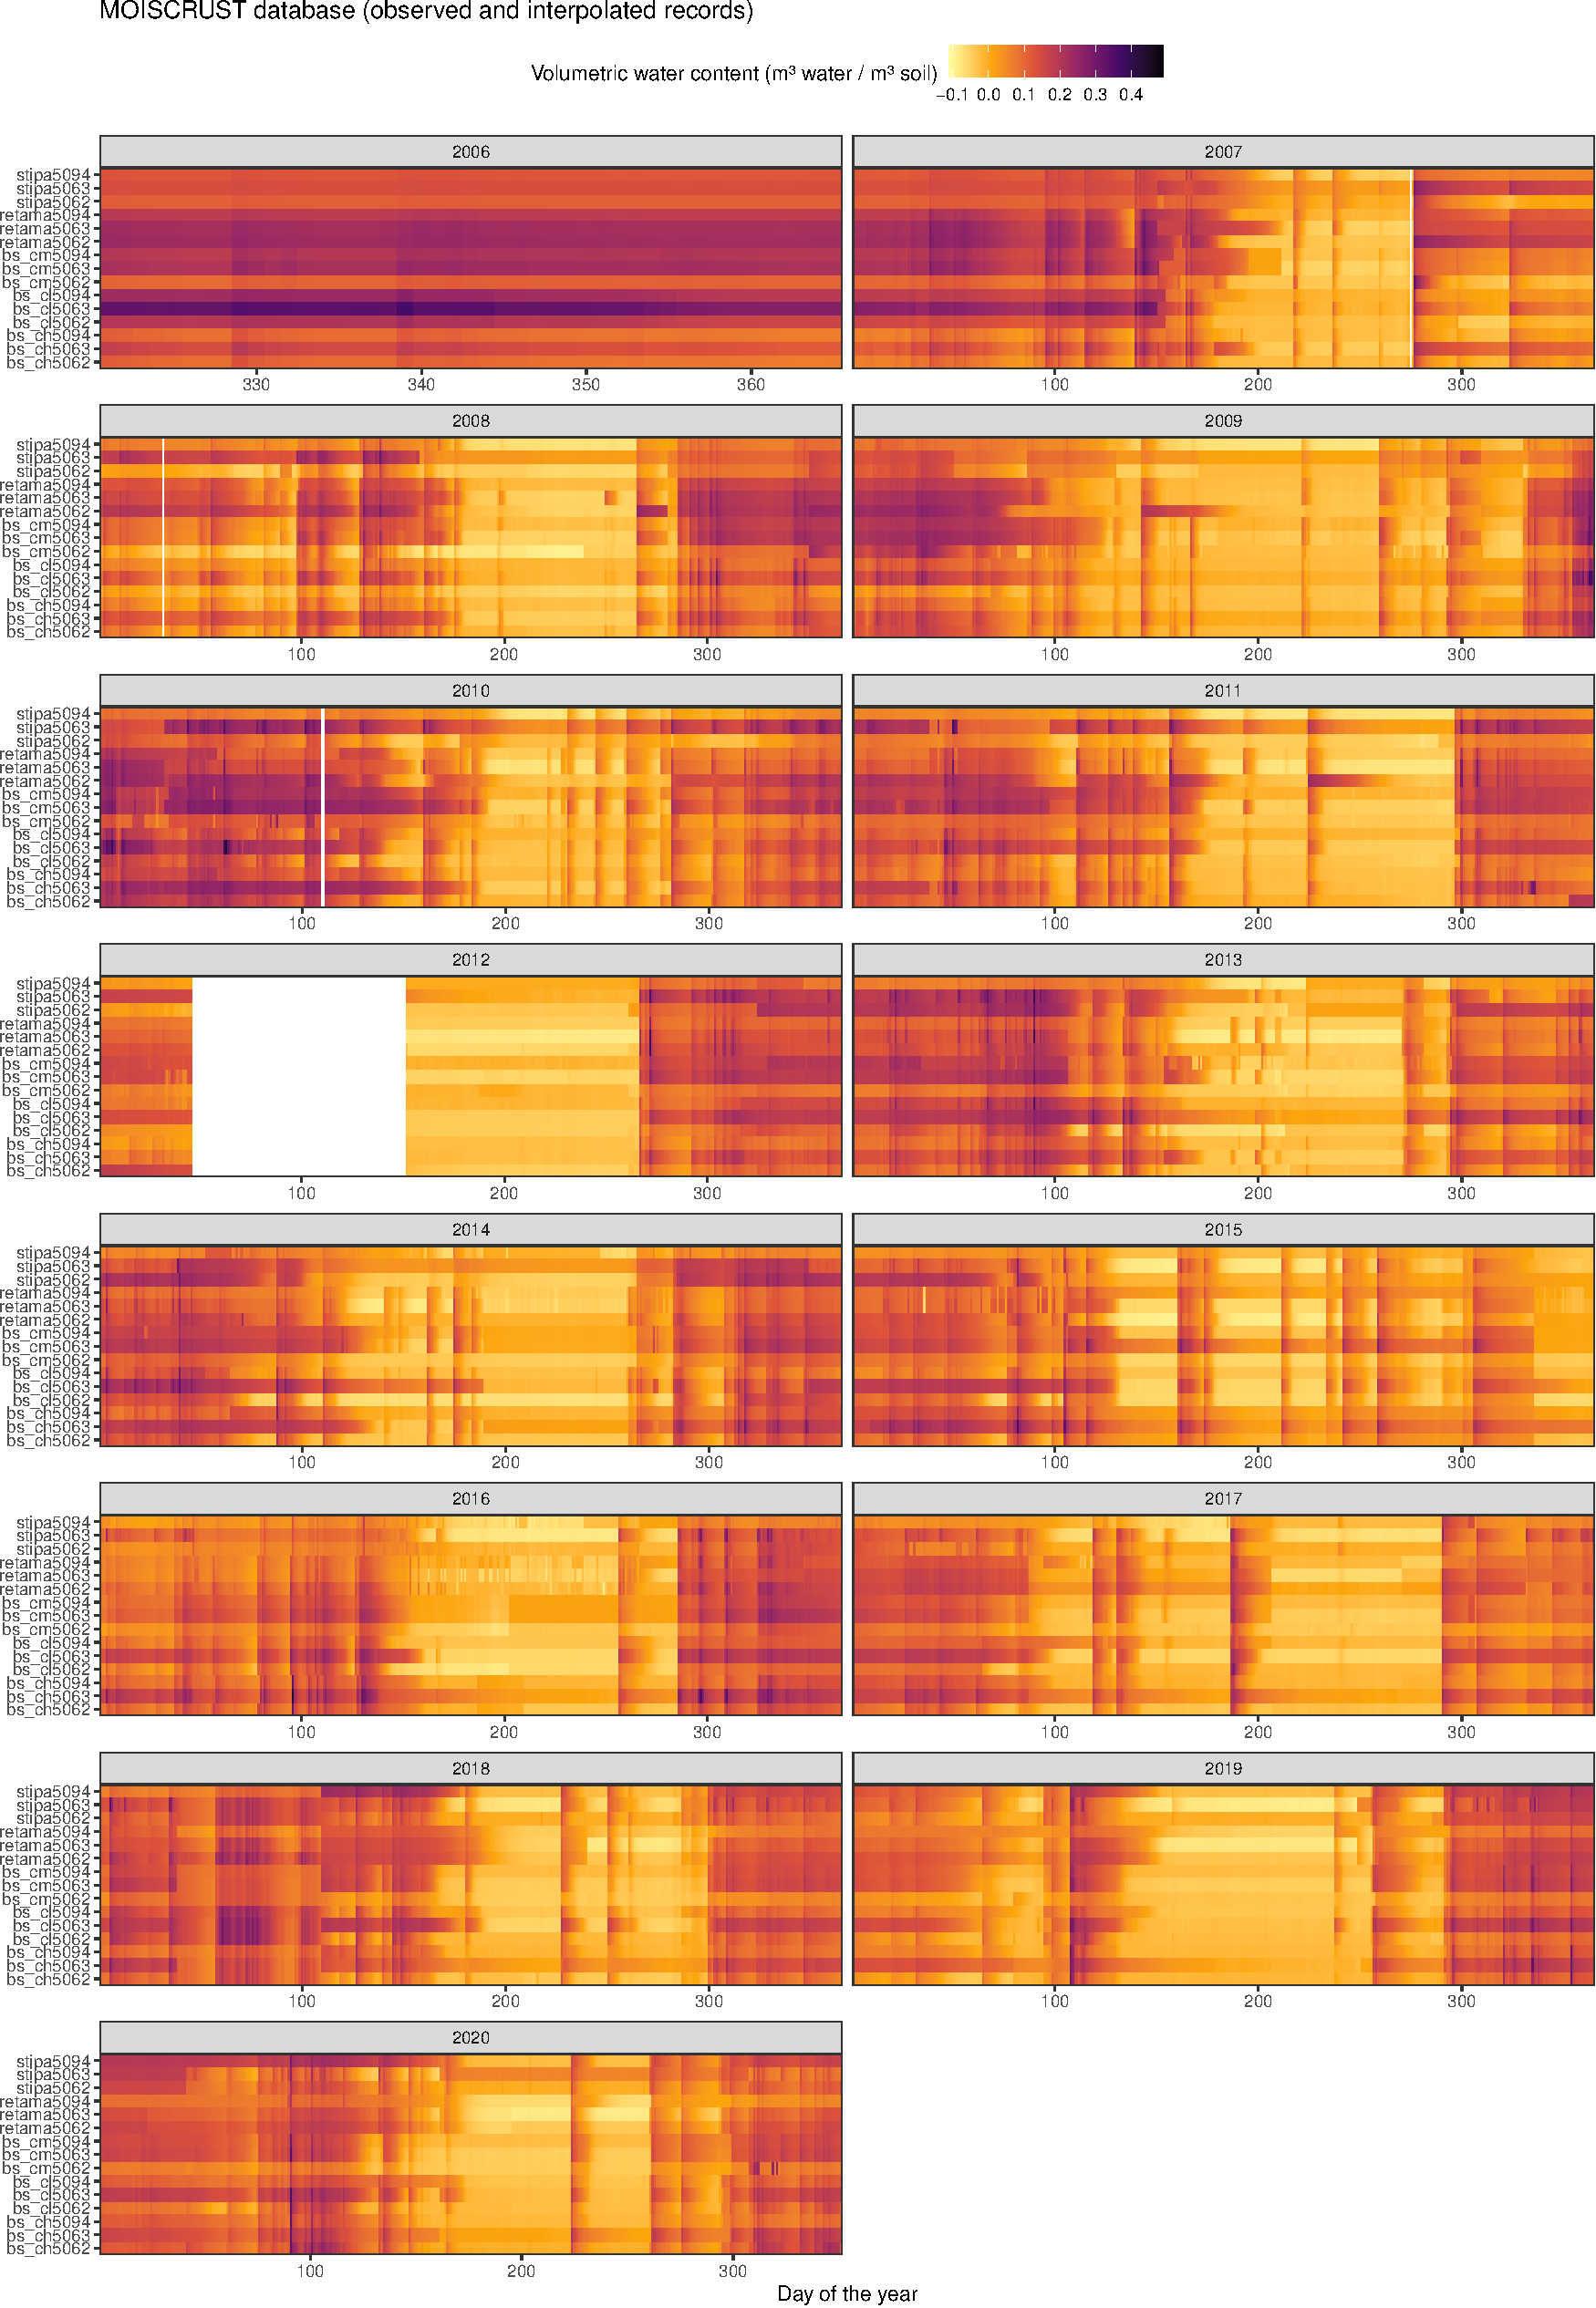
\includegraphics{moiscrust_files/figure-latex/unnamed-chunk-29-1.pdf}

The plot above represents both observed and interpolated values, without
a clear differentiation between each type. To provide an indicator of
imputation quality, the imputation algorithm also generated a new column
named \emph{interpolation\_quality}, where the observations are marked
with the flag ``observation'', the imputed data where \emph{x} and
\emph{y} shared more than 20\% of valid cases and had an R² higher than
0.85 are marked with the flag ``acceptable'', and the imputed data below
these thresholds are marked with the flag ``poor''. The plot below shows
the values of these flags for each sensor and time, year per year.

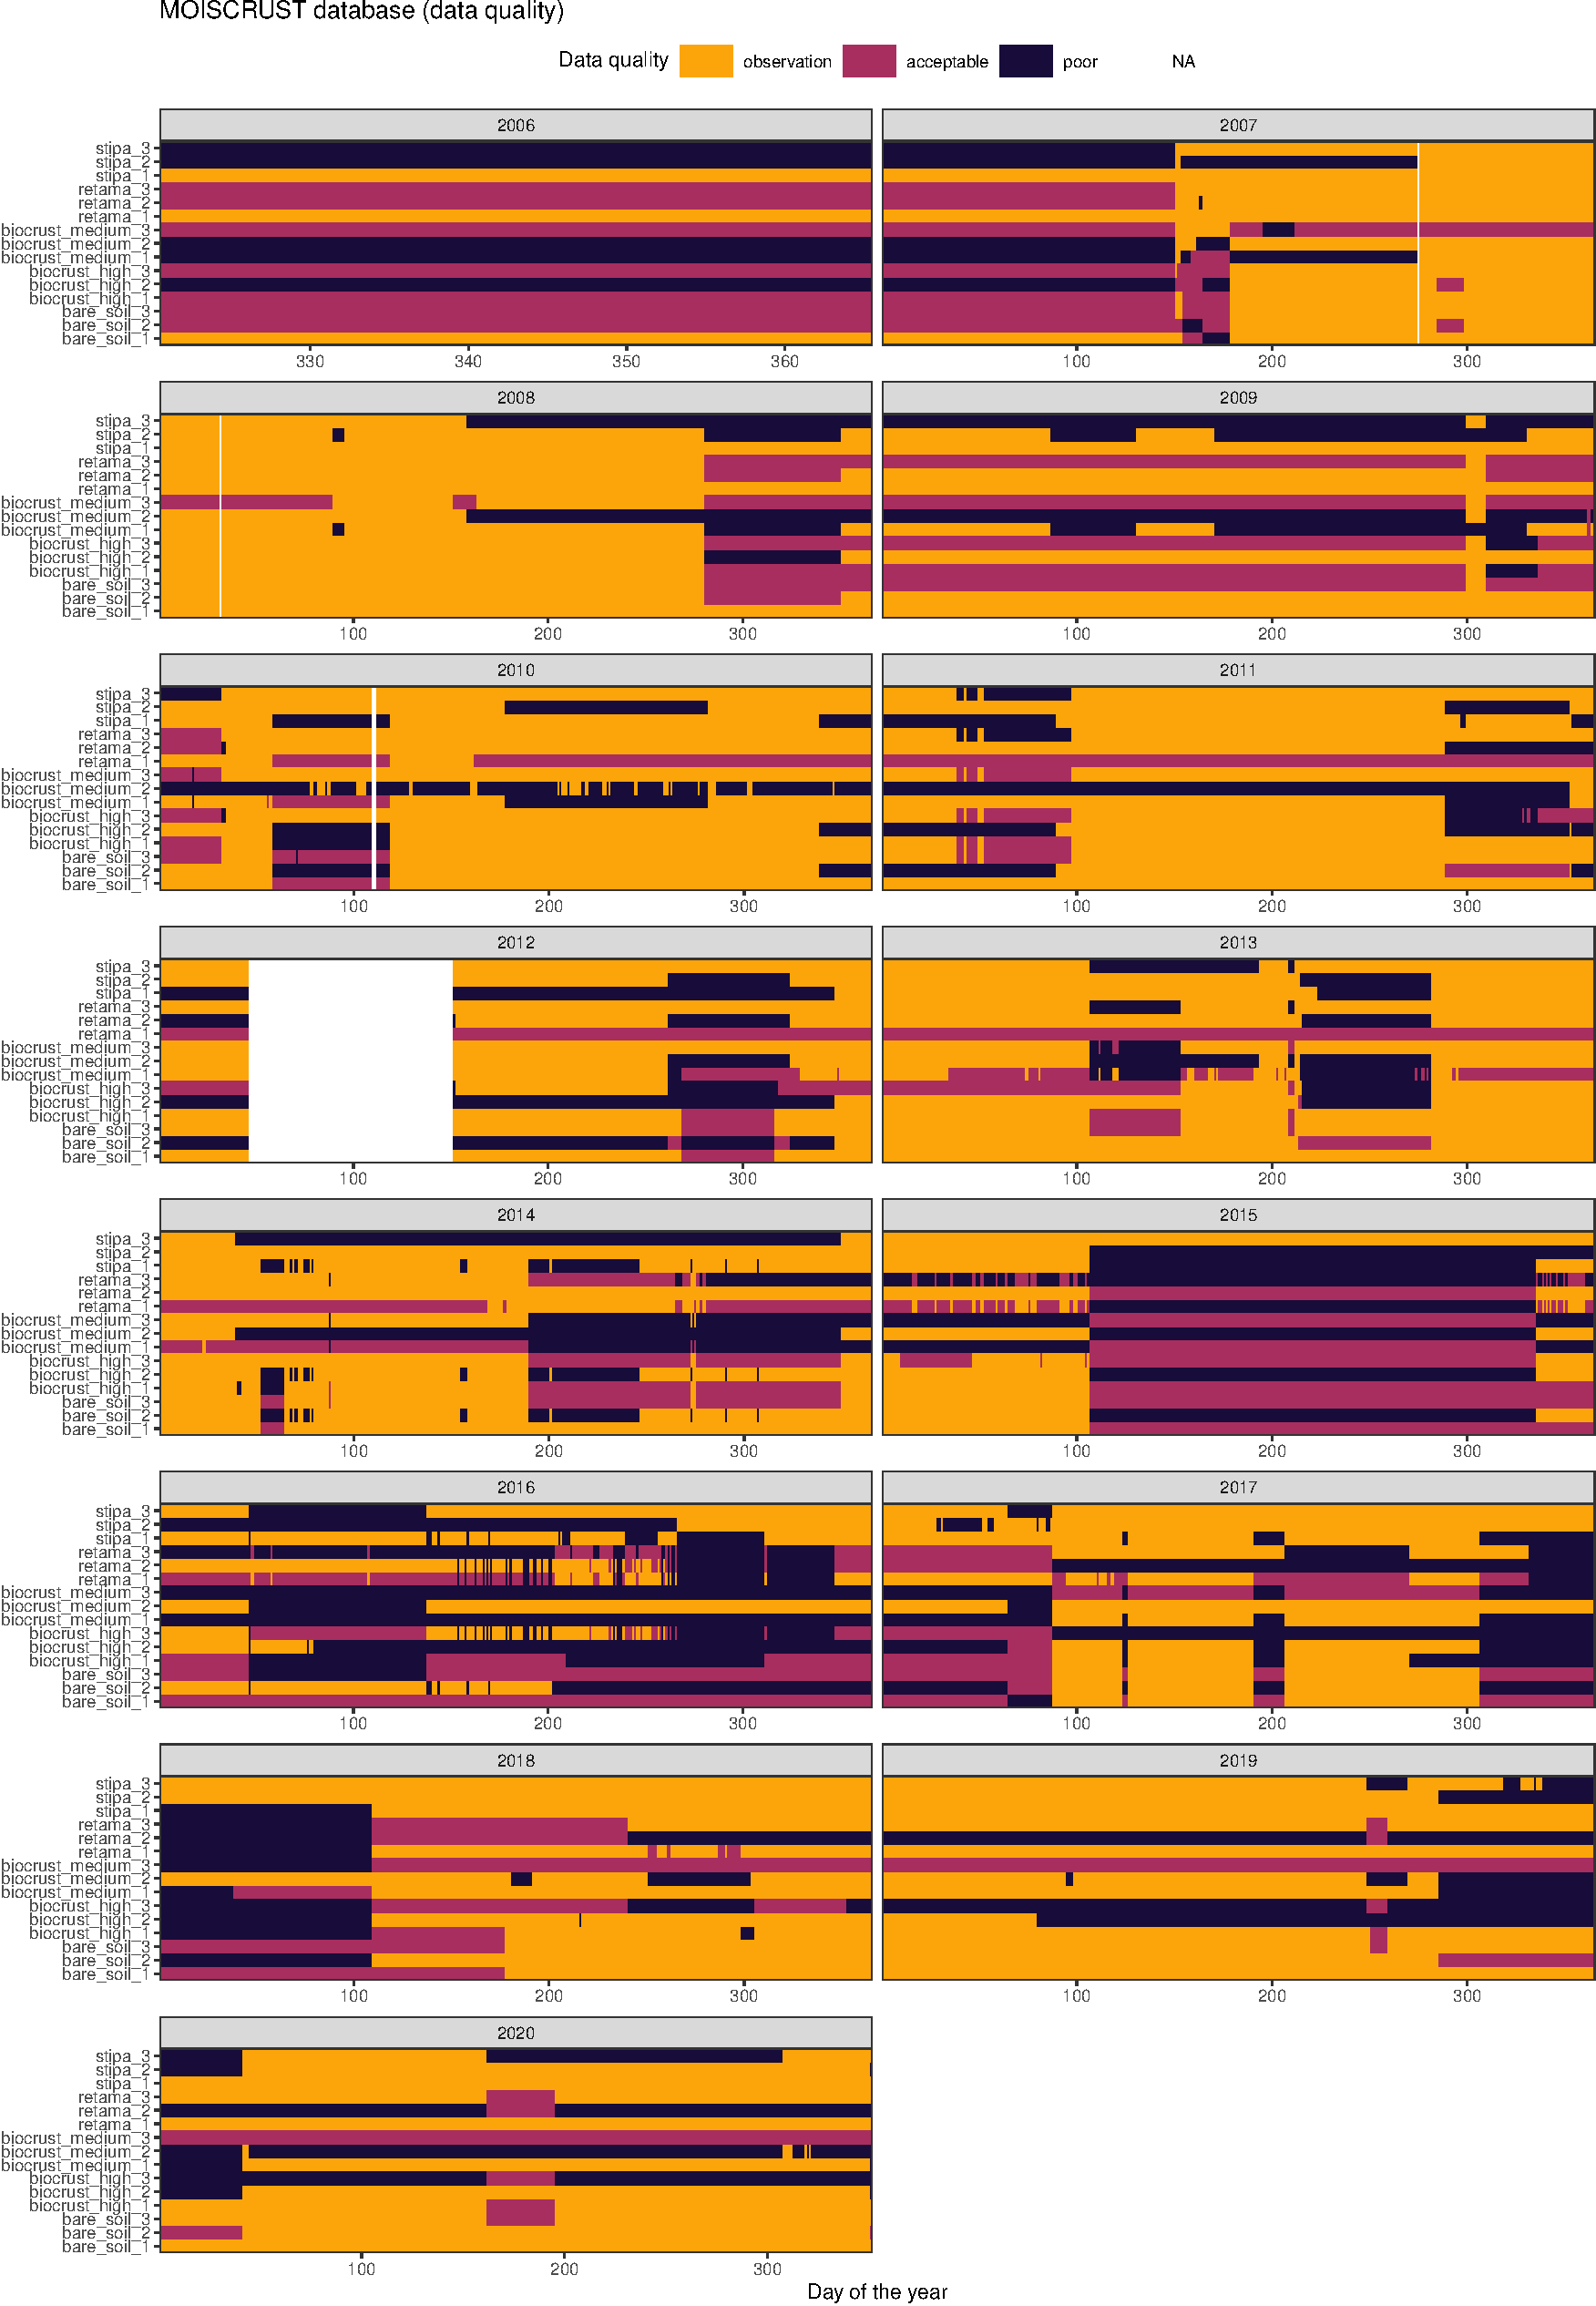
\includegraphics{moiscrust_files/figure-latex/unnamed-chunk-30-1.pdf}

\hypertarget{data-base-format}{%
\section{Data base format}\label{data-base-format}}

The dataset \textbf{moiscrust\_long} is the database in long format
already. Now we can rename it to \textbf{moiscrust}.

\begin{Shaded}
\begin{Highlighting}[]
\NormalTok{moiscrust <-}\StringTok{ }\NormalTok{moiscrust_long}
\end{Highlighting}
\end{Shaded}

The database columns are:

\begin{itemize}
\tightlist
\item
  \emph{date\_time}: date and time in POSIX format.
\item
  \emph{date\_time\_id}: integer, unique ID for each value of
  \emph{date\_time}.
\item
  \emph{date}: date in format year-month-day.
\item
  \emph{time}: time in format hour-minute.
\item
  \emph{year}: integer, year.
\item
  \emph{year\_day}: integer, day of the year.
\item
  \emph{month}: integer, month number.
\item
  \emph{week}: integer, week of the year.
\item
  \emph{week\_day}: integer, day of the week.
\item
  \emph{sensor}: character, sensor name.
\item
  \emph{soil\_moisture}: numeric, soil moisture value in
  \(m^{3} water /m^{3} soil\).
\item
  \emph{interpolated}: boolean, \emph{TRUE} for interpolated records and
  \emph{FALSE} for observations.
\item
  \emph{model\_estimate}: numeric, prediction of the linear model.
\item
  \emph{model\_ci\_lower}: numeric, lower bound of the confidence
  interval of the estimate.
\item
  \emph{model\_ci\_upper}: numeric, upper bound of the confidence
  interval of the estimate.
\item
  \emph{model\_predictor}: character, name of the sensor used as
  predictor in the linear model.
\item
  \emph{same\_microsite}: boolean, \emph{TRUE} if the sensor and its
  predictor are in the same group (``stipa'', ``retama'',
  ``biocrust\_low'', ``biocrust\_medium'', ``biocrust\_high'').
\item
  \emph{sensors\_r\_squared}: numeric, R squared between \emph{sensor}
  and \emph{model\_predictor}.
\item
  \emph{sensors\_shared\_valid\_percent}: numeric, percentage of shared
  valid cases between \emph{sensor} and \emph{model\_predictor}, taking
  the total number of values in \emph{date\_time\_id} as reference.
\item
  \emph{selection\_score}: numeric, value used to select the
  \emph{model\_predictor}, based on the sum of \emph{same\_microsite}
  (100 if \emph{TRUE} and 0 if \emph{FALSE}), \emph{sensors\_r\_squared}
  multiplied by 100, and \emph{sensors\_shared\_valid\_percent}.
\item
  \emph{interpolation\_quality}: character, with the values
  ``observation'' for observations, ``acceptable'' for interpolated
  values where \emph{sensors\_r\_squared} is higher than 0.85 and
  \emph{sensors\_shared\_valid\_percent} is higher than 20, and ``poor''
  for interpolated values below at least one of these thresholds.
\end{itemize}

\hypertarget{saving-the-data-base-in-different-formats}{%
\subsection{Saving the data base in different
formats}\label{saving-the-data-base-in-different-formats}}

To expand its usability as much as possible, we provide the data in four
different formats: .RData, .csv, .xlsx, and SQLite.

\begin{Shaded}
\begin{Highlighting}[]
\CommentTok{#if the zip file does not exists, creates database directory and populates it}
\ControlFlowTok{if}\NormalTok{(}\OperatorTok{!}\KeywordTok{file.exists}\NormalTok{(}\StringTok{"database.zip"}\NormalTok{))\{}
  
  \KeywordTok{dir.create}\NormalTok{(}\StringTok{"database"}\NormalTok{)}
  
  \CommentTok{#save as RData}
  \KeywordTok{save}\NormalTok{(}
\NormalTok{    moiscrust, }
    \DataTypeTok{file =} \StringTok{"database/moiscrust.RData"}
\NormalTok{  )}
  
  \CommentTok{#save as csv}
\NormalTok{  readr}\OperatorTok{::}\KeywordTok{write_excel_csv}\NormalTok{(}
    \DataTypeTok{x =}\NormalTok{ moiscrust,}
    \DataTypeTok{file =} \StringTok{"database/moiscrust.csv"}
\NormalTok{  )}
  
  \CommentTok{#save as excel file}
\NormalTok{  writexl}\OperatorTok{::}\KeywordTok{write_xlsx}\NormalTok{(}
    \DataTypeTok{x =}\NormalTok{ moiscrust,}
    \DataTypeTok{path =} \StringTok{"database/moiscrust.xlsx"}
\NormalTok{  )}
  
  \CommentTok{#save as SQLite}
\NormalTok{  db.driver <-}\StringTok{ }\NormalTok{DBI}\OperatorTok{::}\KeywordTok{dbDriver}\NormalTok{(}\StringTok{"SQLite"}\NormalTok{)}
\NormalTok{  db.connection <-}\StringTok{  }\NormalTok{DBI}\OperatorTok{::}\KeywordTok{dbConnect}\NormalTok{(}
\NormalTok{    db.driver, }
    \DataTypeTok{dbname =} \StringTok{"database/moiscrust.db"}
\NormalTok{    )}
\NormalTok{  DBI}\OperatorTok{::}\KeywordTok{dbWriteTable}\NormalTok{(}
\NormalTok{    db.connection, }
    \StringTok{"moiscrust"}\NormalTok{, }
\NormalTok{    moiscrust, }
    \DataTypeTok{overwrite =} \OtherTok{TRUE}
\NormalTok{    )}
\NormalTok{  DBI}\OperatorTok{::}\KeywordTok{dbDisconnect}\NormalTok{(db.connection)}
  
  \CommentTok{#compressing the file}
\NormalTok{  zip}\OperatorTok{::}\KeywordTok{zip}\NormalTok{(}
    \DataTypeTok{zipfile =} \StringTok{"database.zip"}\NormalTok{,}
    \DataTypeTok{files =} \StringTok{"database"}
\NormalTok{  )}
  
  \CommentTok{#removing the database folder}
  \KeywordTok{unlink}\NormalTok{(}
    \StringTok{"database"}\NormalTok{, }
    \DataTypeTok{recursive =} \OtherTok{TRUE}
\NormalTok{    )}
  
  \CommentTok{#clean the R environment}
  \KeywordTok{rm}\NormalTok{(}
\NormalTok{    db.connection,}
\NormalTok{    db.driver,}
\NormalTok{    moiscrust}
\NormalTok{    )}
  
\NormalTok{\}}
\end{Highlighting}
\end{Shaded}

\end{document}
